% Options for packages loaded elsewhere
\PassOptionsToPackage{unicode}{hyperref}
\PassOptionsToPackage{hyphens}{url}
%
\documentclass[
]{article}
\usepackage{amsmath,amssymb}
\usepackage{iftex}
\ifPDFTeX
  \usepackage[T1]{fontenc}
  \usepackage[utf8]{inputenc}
  \usepackage{textcomp} % provide euro and other symbols
\else % if luatex or xetex
  \usepackage{unicode-math} % this also loads fontspec
  \defaultfontfeatures{Scale=MatchLowercase}
  \defaultfontfeatures[\rmfamily]{Ligatures=TeX,Scale=1}
\fi
\usepackage{lmodern}
\ifPDFTeX\else
  % xetex/luatex font selection
\fi
% Use upquote if available, for straight quotes in verbatim environments
\IfFileExists{upquote.sty}{\usepackage{upquote}}{}
\IfFileExists{microtype.sty}{% use microtype if available
  \usepackage[]{microtype}
  \UseMicrotypeSet[protrusion]{basicmath} % disable protrusion for tt fonts
}{}
\makeatletter
\@ifundefined{KOMAClassName}{% if non-KOMA class
  \IfFileExists{parskip.sty}{%
    \usepackage{parskip}
  }{% else
    \setlength{\parindent}{0pt}
    \setlength{\parskip}{6pt plus 2pt minus 1pt}}
}{% if KOMA class
  \KOMAoptions{parskip=half}}
\makeatother
\usepackage{xcolor}
\usepackage[margin=1in]{geometry}
\usepackage{color}
\usepackage{fancyvrb}
\newcommand{\VerbBar}{|}
\newcommand{\VERB}{\Verb[commandchars=\\\{\}]}
\DefineVerbatimEnvironment{Highlighting}{Verbatim}{commandchars=\\\{\}}
% Add ',fontsize=\small' for more characters per line
\usepackage{framed}
\definecolor{shadecolor}{RGB}{248,248,248}
\newenvironment{Shaded}{\begin{snugshade}}{\end{snugshade}}
\newcommand{\AlertTok}[1]{\textcolor[rgb]{0.94,0.16,0.16}{#1}}
\newcommand{\AnnotationTok}[1]{\textcolor[rgb]{0.56,0.35,0.01}{\textbf{\textit{#1}}}}
\newcommand{\AttributeTok}[1]{\textcolor[rgb]{0.13,0.29,0.53}{#1}}
\newcommand{\BaseNTok}[1]{\textcolor[rgb]{0.00,0.00,0.81}{#1}}
\newcommand{\BuiltInTok}[1]{#1}
\newcommand{\CharTok}[1]{\textcolor[rgb]{0.31,0.60,0.02}{#1}}
\newcommand{\CommentTok}[1]{\textcolor[rgb]{0.56,0.35,0.01}{\textit{#1}}}
\newcommand{\CommentVarTok}[1]{\textcolor[rgb]{0.56,0.35,0.01}{\textbf{\textit{#1}}}}
\newcommand{\ConstantTok}[1]{\textcolor[rgb]{0.56,0.35,0.01}{#1}}
\newcommand{\ControlFlowTok}[1]{\textcolor[rgb]{0.13,0.29,0.53}{\textbf{#1}}}
\newcommand{\DataTypeTok}[1]{\textcolor[rgb]{0.13,0.29,0.53}{#1}}
\newcommand{\DecValTok}[1]{\textcolor[rgb]{0.00,0.00,0.81}{#1}}
\newcommand{\DocumentationTok}[1]{\textcolor[rgb]{0.56,0.35,0.01}{\textbf{\textit{#1}}}}
\newcommand{\ErrorTok}[1]{\textcolor[rgb]{0.64,0.00,0.00}{\textbf{#1}}}
\newcommand{\ExtensionTok}[1]{#1}
\newcommand{\FloatTok}[1]{\textcolor[rgb]{0.00,0.00,0.81}{#1}}
\newcommand{\FunctionTok}[1]{\textcolor[rgb]{0.13,0.29,0.53}{\textbf{#1}}}
\newcommand{\ImportTok}[1]{#1}
\newcommand{\InformationTok}[1]{\textcolor[rgb]{0.56,0.35,0.01}{\textbf{\textit{#1}}}}
\newcommand{\KeywordTok}[1]{\textcolor[rgb]{0.13,0.29,0.53}{\textbf{#1}}}
\newcommand{\NormalTok}[1]{#1}
\newcommand{\OperatorTok}[1]{\textcolor[rgb]{0.81,0.36,0.00}{\textbf{#1}}}
\newcommand{\OtherTok}[1]{\textcolor[rgb]{0.56,0.35,0.01}{#1}}
\newcommand{\PreprocessorTok}[1]{\textcolor[rgb]{0.56,0.35,0.01}{\textit{#1}}}
\newcommand{\RegionMarkerTok}[1]{#1}
\newcommand{\SpecialCharTok}[1]{\textcolor[rgb]{0.81,0.36,0.00}{\textbf{#1}}}
\newcommand{\SpecialStringTok}[1]{\textcolor[rgb]{0.31,0.60,0.02}{#1}}
\newcommand{\StringTok}[1]{\textcolor[rgb]{0.31,0.60,0.02}{#1}}
\newcommand{\VariableTok}[1]{\textcolor[rgb]{0.00,0.00,0.00}{#1}}
\newcommand{\VerbatimStringTok}[1]{\textcolor[rgb]{0.31,0.60,0.02}{#1}}
\newcommand{\WarningTok}[1]{\textcolor[rgb]{0.56,0.35,0.01}{\textbf{\textit{#1}}}}
\usepackage{graphicx}
\makeatletter
\def\maxwidth{\ifdim\Gin@nat@width>\linewidth\linewidth\else\Gin@nat@width\fi}
\def\maxheight{\ifdim\Gin@nat@height>\textheight\textheight\else\Gin@nat@height\fi}
\makeatother
% Scale images if necessary, so that they will not overflow the page
% margins by default, and it is still possible to overwrite the defaults
% using explicit options in \includegraphics[width, height, ...]{}
\setkeys{Gin}{width=\maxwidth,height=\maxheight,keepaspectratio}
% Set default figure placement to htbp
\makeatletter
\def\fps@figure{htbp}
\makeatother
\setlength{\emergencystretch}{3em} % prevent overfull lines
\providecommand{\tightlist}{%
  \setlength{\itemsep}{0pt}\setlength{\parskip}{0pt}}
\setcounter{secnumdepth}{-\maxdimen} % remove section numbering
\ifLuaTeX
  \usepackage{selnolig}  % disable illegal ligatures
\fi
\usepackage{bookmark}
\IfFileExists{xurl.sty}{\usepackage{xurl}}{} % add URL line breaks if available
\urlstyle{same}
\hypersetup{
  pdftitle={Project Network-based Data Analysis},
  pdfauthor={Annalisa Xamin},
  hidelinks,
  pdfcreator={LaTeX via pandoc}}

\title{Project Network-based Data Analysis}
\author{Annalisa Xamin}
\date{}

\begin{document}
\maketitle

{
\setcounter{tocdepth}{2}
\tableofcontents
}
\begin{center}\rule{0.5\linewidth}{0.5pt}\end{center}

\subsection{Install and load R
packages}\label{install-and-load-r-packages}

\begin{Shaded}
\begin{Highlighting}[]
\ControlFlowTok{if}\NormalTok{ (}\SpecialCharTok{!}\FunctionTok{require}\NormalTok{(}\StringTok{"BiocManager"}\NormalTok{, }\AttributeTok{quietly =} \ConstantTok{TRUE}\NormalTok{))}
    \FunctionTok{install.packages}\NormalTok{(}\StringTok{"BiocManager"}\NormalTok{)}

\ControlFlowTok{if}\NormalTok{ (}\SpecialCharTok{!}\FunctionTok{require}\NormalTok{(}\StringTok{"GEOquery"}\NormalTok{, }\AttributeTok{quietly =} \ConstantTok{TRUE}\NormalTok{))}
\NormalTok{    BiocManager}\SpecialCharTok{::}\FunctionTok{install}\NormalTok{(}\StringTok{"GEOquery"}\NormalTok{) }

\ControlFlowTok{if}\NormalTok{ (}\SpecialCharTok{!}\FunctionTok{require}\NormalTok{(}\StringTok{"rScudo"}\NormalTok{, }\AttributeTok{quietly =} \ConstantTok{TRUE}\NormalTok{))}
\NormalTok{    BiocManager}\SpecialCharTok{::}\FunctionTok{install}\NormalTok{(}\StringTok{"rScudo"}\NormalTok{) }

\FunctionTok{library}\NormalTok{(tidyverse)}
\FunctionTok{library}\NormalTok{(dplyr)}
\FunctionTok{library}\NormalTok{(GEOquery)}
\FunctionTok{library}\NormalTok{(rScudo)}
\FunctionTok{library}\NormalTok{(plotly)}
\FunctionTok{library}\NormalTok{(sessioninfo)}
\FunctionTok{library}\NormalTok{(ggplot2)}
\FunctionTok{library}\NormalTok{(factoextra)}
\FunctionTok{library}\NormalTok{(useful)}
\FunctionTok{library}\NormalTok{(umap)}

\NormalTok{my\_colors }\OtherTok{\textless{}{-}} \FunctionTok{c}\NormalTok{(}\StringTok{"\#2e005d"}\NormalTok{, }\StringTok{"\#5c008b"}\NormalTok{, }\StringTok{"\#8e008b"}\NormalTok{, }\StringTok{"\#ff8300"}\NormalTok{, }\StringTok{"\#ff6200"}\NormalTok{, }\StringTok{"\#d1105a"}\NormalTok{, }\StringTok{"\#05a8aa"}\NormalTok{)}
\end{Highlighting}
\end{Shaded}

\section{R session information}\label{r-session-information}

Print the R session information for reproducibility.

\begin{Shaded}
\begin{Highlighting}[]
\FunctionTok{print}\NormalTok{(}\StringTok{\textquotesingle{}Reproducibility information:\textquotesingle{}}\NormalTok{) }
\end{Highlighting}
\end{Shaded}

\begin{verbatim}
## [1] "Reproducibility information:"
\end{verbatim}

\begin{Shaded}
\begin{Highlighting}[]
\FunctionTok{Sys.time}\NormalTok{()}
\end{Highlighting}
\end{Shaded}

\begin{verbatim}
## [1] "2024-10-16 10:52:25 CEST"
\end{verbatim}

\begin{Shaded}
\begin{Highlighting}[]
\FunctionTok{proc.time}\NormalTok{()}
\end{Highlighting}
\end{Shaded}

\begin{verbatim}
##    user  system elapsed 
##   1.701   0.149   2.319
\end{verbatim}

\begin{Shaded}
\begin{Highlighting}[]
\FunctionTok{options}\NormalTok{(}\AttributeTok{width =} \DecValTok{120}\NormalTok{)}
\FunctionTok{session\_info}\NormalTok{()}
\end{Highlighting}
\end{Shaded}

\begin{verbatim}
## - Session info -------------------------------------------------------------------------------------------------------
##  setting  value
##  version  R version 4.4.0 (2024-04-24)
##  os       macOS 15.0.1
##  system   aarch64, darwin23.4.0
##  ui       unknown
##  language (EN)
##  collate  en_US.UTF-8
##  ctype    en_US.UTF-8
##  tz       Europe/Rome
##  date     2024-10-16
##  pandoc   3.1.11 @ /Applications/RStudio.app/Contents/Resources/app/quarto/bin/tools/aarch64/ (via rmarkdown)
## 
## - Packages -----------------------------------------------------------------------------------------------------------
##  package      * version  date (UTC) lib source
##  askpass        1.2.0    2023-09-03 [1] CRAN (R 4.4.0)
##  Biobase      * 2.64.0   2024-04-30 [1] Bioconductor 3.19 (R 4.4.0)
##  BiocGenerics * 0.50.0   2024-04-30 [1] Bioconductor 3.19 (R 4.4.0)
##  BiocManager  * 1.30.25  2024-08-28 [1] CRAN (R 4.4.0)
##  cli            3.6.3    2024-06-21 [1] CRAN (R 4.4.0)
##  colorspace     2.1-1    2024-07-26 [1] CRAN (R 4.4.0)
##  data.table     1.16.0   2024-08-27 [1] CRAN (R 4.4.0)
##  digest         0.6.37   2024-08-19 [1] CRAN (R 4.4.0)
##  dplyr        * 1.1.4    2023-11-17 [1] CRAN (R 4.4.0)
##  evaluate       0.24.0   2024-06-10 [1] CRAN (R 4.4.0)
##  factoextra   * 1.0.7    2020-04-01 [1] CRAN (R 4.4.0)
##  fansi          1.0.6    2023-12-08 [1] CRAN (R 4.4.0)
##  fastmap        1.2.0    2024-05-15 [1] CRAN (R 4.4.0)
##  forcats      * 1.0.0    2023-01-29 [1] CRAN (R 4.4.0)
##  generics       0.1.3    2022-07-05 [1] CRAN (R 4.4.0)
##  GEOquery     * 2.72.0   2024-04-30 [1] Bioconductor 3.19 (R 4.4.0)
##  ggplot2      * 3.5.1    2024-04-23 [1] CRAN (R 4.4.0)
##  ggrepel        0.9.6    2024-09-07 [1] CRAN (R 4.4.0)
##  glue           1.7.0    2024-01-09 [1] CRAN (R 4.4.0)
##  gtable         0.3.5    2024-04-22 [1] CRAN (R 4.4.0)
##  hms            1.1.3    2023-03-21 [1] CRAN (R 4.4.0)
##  htmltools      0.5.8.1  2024-04-04 [1] CRAN (R 4.4.0)
##  htmlwidgets    1.6.4    2023-12-06 [1] CRAN (R 4.4.0)
##  httr           1.4.7    2023-08-15 [1] CRAN (R 4.4.0)
##  jsonlite       1.8.8    2023-12-04 [1] CRAN (R 4.4.0)
##  knitr          1.48     2024-07-07 [1] CRAN (R 4.4.0)
##  lattice        0.22-6   2024-03-20 [2] CRAN (R 4.4.0)
##  lazyeval       0.2.2    2019-03-15 [1] CRAN (R 4.4.0)
##  lifecycle      1.0.4    2023-11-07 [1] CRAN (R 4.4.0)
##  limma          3.60.4   2024-07-17 [1] Bioconductor 3.19 (R 4.4.0)
##  lubridate    * 1.9.3    2023-09-27 [1] CRAN (R 4.4.0)
##  magrittr       2.0.3    2022-03-30 [1] CRAN (R 4.4.0)
##  Matrix         1.7-0    2024-03-22 [2] CRAN (R 4.4.0)
##  munsell        0.5.1    2024-04-01 [1] CRAN (R 4.4.0)
##  openssl        2.2.1    2024-08-16 [1] CRAN (R 4.4.0)
##  pillar         1.9.0    2023-03-22 [1] CRAN (R 4.4.0)
##  pkgconfig      2.0.3    2019-09-22 [1] CRAN (R 4.4.0)
##  plotly       * 4.10.4   2024-01-13 [1] CRAN (R 4.4.0)
##  plyr           1.8.9    2023-10-02 [1] CRAN (R 4.4.0)
##  png            0.1-8    2022-11-29 [1] CRAN (R 4.4.0)
##  purrr        * 1.0.2    2023-08-10 [1] CRAN (R 4.4.0)
##  R6             2.5.1    2021-08-19 [1] CRAN (R 4.4.0)
##  Rcpp           1.0.13   2024-07-17 [1] CRAN (R 4.4.0)
##  readr        * 2.1.5    2024-01-10 [1] CRAN (R 4.4.0)
##  reticulate     1.39.0   2024-09-05 [1] CRAN (R 4.4.0)
##  rlang          1.1.4    2024-06-04 [1] CRAN (R 4.4.0)
##  rmarkdown      2.28     2024-08-17 [1] CRAN (R 4.4.0)
##  rScudo       * 1.20.0   2024-04-30 [1] Bioconductor 3.19 (R 4.4.0)
##  RSpectra       0.16-2   2024-07-18 [1] CRAN (R 4.4.0)
##  rstudioapi     0.16.0   2024-03-24 [1] CRAN (R 4.4.0)
##  scales         1.3.0    2023-11-28 [1] CRAN (R 4.4.0)
##  sessioninfo  * 1.2.2    2021-12-06 [1] CRAN (R 4.4.0)
##  statmod        1.5.0    2023-01-06 [1] CRAN (R 4.4.0)
##  stringi        1.8.4    2024-05-06 [1] CRAN (R 4.4.0)
##  stringr      * 1.5.1    2023-11-14 [1] CRAN (R 4.4.0)
##  tibble       * 3.2.1    2023-03-20 [1] CRAN (R 4.4.0)
##  tidyr        * 1.3.1    2024-01-24 [1] CRAN (R 4.4.0)
##  tidyselect     1.2.1    2024-03-11 [1] CRAN (R 4.4.0)
##  tidyverse    * 2.0.0    2023-02-22 [1] CRAN (R 4.4.0)
##  timechange     0.3.0    2024-01-18 [1] CRAN (R 4.4.0)
##  tzdb           0.4.0    2023-05-12 [1] CRAN (R 4.4.0)
##  umap         * 0.2.10.0 2023-02-01 [1] CRAN (R 4.4.0)
##  useful       * 1.2.6.1  2023-10-24 [1] CRAN (R 4.4.0)
##  utf8           1.2.4    2023-10-22 [1] CRAN (R 4.4.0)
##  vctrs          0.6.5    2023-12-01 [1] CRAN (R 4.4.0)
##  viridisLite    0.4.2    2023-05-02 [1] CRAN (R 4.4.0)
##  withr          3.0.1    2024-07-31 [1] CRAN (R 4.4.0)
##  xfun           0.47     2024-08-17 [1] CRAN (R 4.4.0)
##  xml2           1.3.6    2023-12-04 [1] CRAN (R 4.4.0)
##  yaml           2.3.10   2024-07-26 [1] CRAN (R 4.4.0)
## 
##  [1] /opt/homebrew/lib/R/4.4/site-library
##  [2] /opt/homebrew/Cellar/r/4.4.0/lib/R/library
## 
## ----------------------------------------------------------------------------------------------------------------------
\end{verbatim}

\section{Data selection}\label{data-selection}

The analysis will use the dataset
\href{https://www.ncbi.nlm.nih.gov/geo/query/acc.cgi?acc=GSE20437}{GSE20437}
obtained from GEO.The dataset is generated from Affymetrix HU133A
microarrays and contains 42 tissue samples.

In detail, the data includes:

\begin{itemize}
\item
  18 reduction mammoplasty (RM) breast epithelium samples,
\item
  18 histologically normal (HN) epithelial samples from breast cancer
  patients (9 ER+ and 9 ER-), and
\item
  6 histologically normal epithelial samples from prophylactic
  mastectomy patients.
\end{itemize}

Note that sample numbers correspond to individual patient samples.

\begin{Shaded}
\begin{Highlighting}[]
\CommentTok{\# download the GSE20437 expression data series}
\NormalTok{gse }\OtherTok{\textless{}{-}} \FunctionTok{getGEO}\NormalTok{(}\StringTok{"GSE20437"}\NormalTok{, }\AttributeTok{destdir=} \StringTok{\textquotesingle{}./data/\textquotesingle{}}\NormalTok{, }\AttributeTok{getGPL =}\NormalTok{ F)}
\end{Highlighting}
\end{Shaded}

\begin{Shaded}
\begin{Highlighting}[]
\CommentTok{\# getGEO returns a list of expression objects, but...}
\FunctionTok{length}\NormalTok{(gse) }
\end{Highlighting}
\end{Shaded}

\begin{verbatim}
## [1] 1
\end{verbatim}

\begin{Shaded}
\begin{Highlighting}[]
\CommentTok{\# shows us there is only one object in it. }
\CommentTok{\# We assign it to the same variable.}
\NormalTok{gse }\OtherTok{\textless{}{-}}\NormalTok{ gse[[}\DecValTok{1}\NormalTok{]]}
\end{Highlighting}
\end{Shaded}

\begin{Shaded}
\begin{Highlighting}[]
\CommentTok{\# extract metadata}
\NormalTok{metadata }\OtherTok{\textless{}{-}} \FunctionTok{data.frame}\NormalTok{(gse}\SpecialCharTok{@}\NormalTok{phenoData}\SpecialCharTok{@}\NormalTok{data)}

\CommentTok{\# save metadata to csv file}
\CommentTok{\#write.csv(metadata, file = \textquotesingle{}metadata.csv\textquotesingle{}, row.names = TRUE)}
\end{Highlighting}
\end{Shaded}

\begin{Shaded}
\begin{Highlighting}[]
\NormalTok{p }\OtherTok{\textless{}{-}} \FunctionTok{ggplot}\NormalTok{(metadata, }\FunctionTok{aes}\NormalTok{(}\AttributeTok{x=}\NormalTok{disease.state.ch1, }\AttributeTok{fill=}\NormalTok{specimen.ch1))}\SpecialCharTok{+}
  \FunctionTok{geom\_bar}\NormalTok{()}\SpecialCharTok{+}
  \FunctionTok{scale\_fill\_manual}\NormalTok{(}\AttributeTok{values =}\NormalTok{ my\_colors[}\FunctionTok{c}\NormalTok{(}\DecValTok{1}\NormalTok{,}\DecValTok{4}\NormalTok{,}\DecValTok{6}\NormalTok{,}\DecValTok{7}\NormalTok{)])}
\NormalTok{p }\SpecialCharTok{+} \FunctionTok{labs}\NormalTok{(}\AttributeTok{x =} \StringTok{"Group"}\NormalTok{) }
\end{Highlighting}
\end{Shaded}

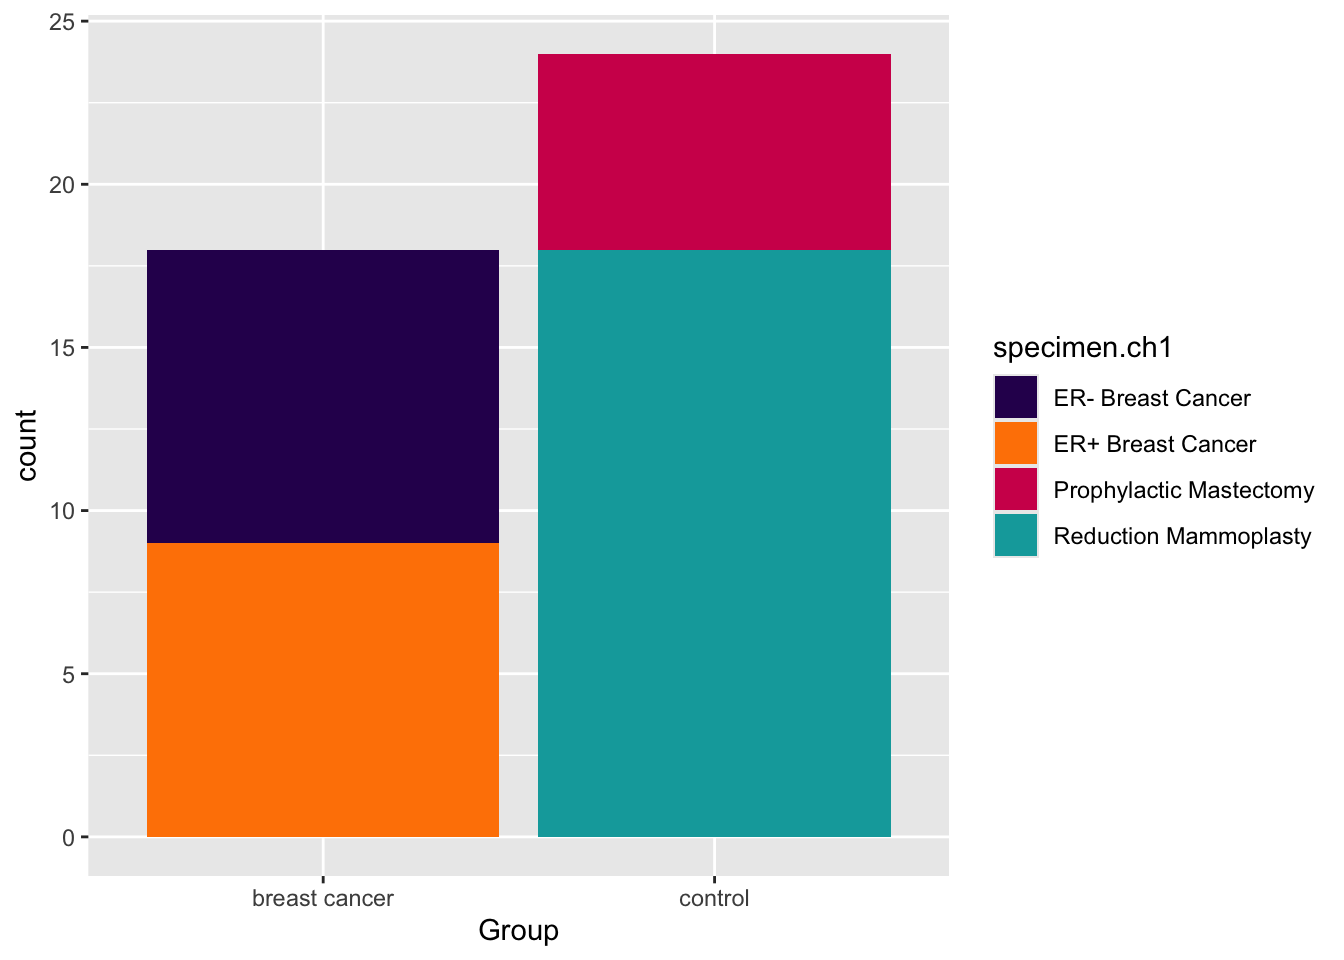
\includegraphics{NBDA_project_files/figure-latex/plot groups-1.pdf}

\section{Exploratory analysis}\label{exploratory-analysis}

\begin{Shaded}
\begin{Highlighting}[]
\CommentTok{\# show what we have:}
\FunctionTok{show}\NormalTok{(gse)}
\end{Highlighting}
\end{Shaded}

\begin{verbatim}
## ExpressionSet (storageMode: lockedEnvironment)
## assayData: 22283 features, 42 samples 
##   element names: exprs 
## protocolData: none
## phenoData
##   sampleNames: GSM512539 GSM512540 ... GSM512580 (42 total)
##   varLabels: title geo_accession ... tissue:ch1 (38 total)
##   varMetadata: labelDescription
## featureData: none
## experimentData: use 'experimentData(object)'
##   pubMedIds: 20197764 
## Annotation: GPL96
\end{verbatim}

The actual expression data are accessible in the \texttt{exprs} section
of \texttt{gse}, an Expression Set and the generic data class that
BioConductor uses for expression data.

\begin{Shaded}
\begin{Highlighting}[]
\FunctionTok{head}\NormalTok{(}\FunctionTok{exprs}\NormalTok{(gse)) }
\end{Highlighting}
\end{Shaded}

\begin{verbatim}
##           GSM512539 GSM512540 GSM512541 GSM512542 GSM512543 GSM512544 GSM512545 GSM512546 GSM512547 GSM512548 GSM512549
## 1007_s_at    2461.4    3435.7    1932.5    2377.7    3055.3    2978.1    2348.5    2963.9    2776.9    3088.9    3033.3
## 1053_at        26.7     159.0      31.2     140.7      69.9      98.5      37.0      59.9      86.7     107.2      64.0
## 117_at         82.6     243.4     150.2      95.1     209.3     103.4      91.2     168.4     162.7     203.2     143.7
## 121_at        942.3     897.5     840.8     870.9     685.4     791.8     886.5     954.2     843.1     775.3     847.6
## 1255_g_at      71.8      87.9      75.4      58.1      31.8      40.3      70.5      43.3      51.6      42.6      74.9
## 1294_at       630.2     571.4     346.3     679.9    1289.3     421.1     417.6     811.6     778.1     393.2     995.4
##           GSM512550 GSM512551 GSM512552 GSM512553 GSM512554 GSM512555 GSM512556 GSM512557 GSM512558 GSM512559 GSM512560
## 1007_s_at    3037.1    3545.8    3322.6    1963.7    3609.6    2078.9    4138.6    4260.7    2453.6    2709.0    2612.5
## 1053_at        82.9      97.7      69.7      82.0      45.6      84.5      31.7      37.4      82.4     204.8     119.3
## 117_at        113.5      80.0     186.4     106.6     145.6     144.4     133.6     278.6     173.0     147.8     186.0
## 121_at        912.2     911.6     862.4     705.0     984.6     853.8     846.8    1273.0     833.6     908.1     806.2
## 1255_g_at      53.7      30.5      15.2      42.5      76.6      88.2      90.6      65.8      25.8      77.5      84.3
## 1294_at       987.7     938.5     924.6     480.8    1054.1     632.0     448.0    1345.2    1248.9     405.7     647.5
##           GSM512561 GSM512562 GSM512563 GSM512564 GSM512565 GSM512566 GSM512567 GSM512568 GSM512569 GSM512570 GSM512571
## 1007_s_at    4340.1    3155.3    2390.3    2738.8    3233.1    2836.6    2915.4    3457.5    2798.7    4370.2    2467.3
## 1053_at        76.7     100.3     115.4      14.1      47.6      77.1      47.1      47.0      83.2      40.2      80.3
## 117_at        168.0      95.2      73.6     122.7     107.6     120.9     143.4      92.5      72.1     131.8     156.4
## 121_at        827.0     629.4     709.2     305.6     877.4     425.7     643.8     771.3     681.1     812.7     533.4
## 1255_g_at      87.9      44.6      59.3      12.0      82.1      59.2      62.2      28.3      97.6       8.1      17.9
## 1294_at      2218.1    1321.1     606.7    1709.9     980.8    1268.4     955.8    1157.5     888.6    1130.8     905.1
##           GSM512572 GSM512573 GSM512574 GSM512575 GSM512576 GSM512577 GSM512578 GSM512579 GSM512580
## 1007_s_at    3669.5    3310.1    3942.2    4520.4    3596.1    2989.0    3164.5    2764.3    4258.5
## 1053_at        24.1       8.8      44.6      54.7      56.7      89.9      63.4      57.0      59.5
## 117_at        165.8     141.6      97.1     132.7     124.3     210.5     131.4      89.6     123.3
## 121_at        746.9    1090.3    1008.7     718.6     988.4     295.9     957.3     630.8     869.2
## 1255_g_at      53.0      39.9      11.0      50.2      60.0      34.3      33.5      61.7      50.4
## 1294_at      1138.5     483.0    1326.5    1179.4     668.3     863.2    1055.5    1287.6    1127.8
\end{verbatim}

To conveniently access the data rows and columns present in
\texttt{exprs(gse)}, this matrix is assigned to its own variable
\texttt{ex}.

\begin{Shaded}
\begin{Highlighting}[]
\CommentTok{\# exprs (gse) is a matrix that we can assign to its own variable, to}
\CommentTok{\# conveniently access the data rows and columns}
\NormalTok{ex }\OtherTok{\textless{}{-}} \FunctionTok{exprs}\NormalTok{(gse)}
\FunctionTok{dim}\NormalTok{(ex) }\CommentTok{\# 42 sample, 22283 genes}
\end{Highlighting}
\end{Shaded}

\begin{verbatim}
## [1] 22283    42
\end{verbatim}

The dataset contains gene expression data of 22283 genes (rows) from 42
patients (columns).

\subsection{Pre-processing}\label{pre-processing}

\begin{Shaded}
\begin{Highlighting}[]
\CommentTok{\# Analyze value distributions}
\FunctionTok{boxplot}\NormalTok{(ex, }\AttributeTok{main =} \StringTok{\textquotesingle{}Boxplot of the data before normalization\textquotesingle{}}\NormalTok{,}
        \AttributeTok{xlab =} \StringTok{"Samples"}\NormalTok{,}
        \AttributeTok{ylab =} \StringTok{"Expression Value"}\NormalTok{,}
        \AttributeTok{varwidth =} \ConstantTok{TRUE}
\NormalTok{        )}
\end{Highlighting}
\end{Shaded}

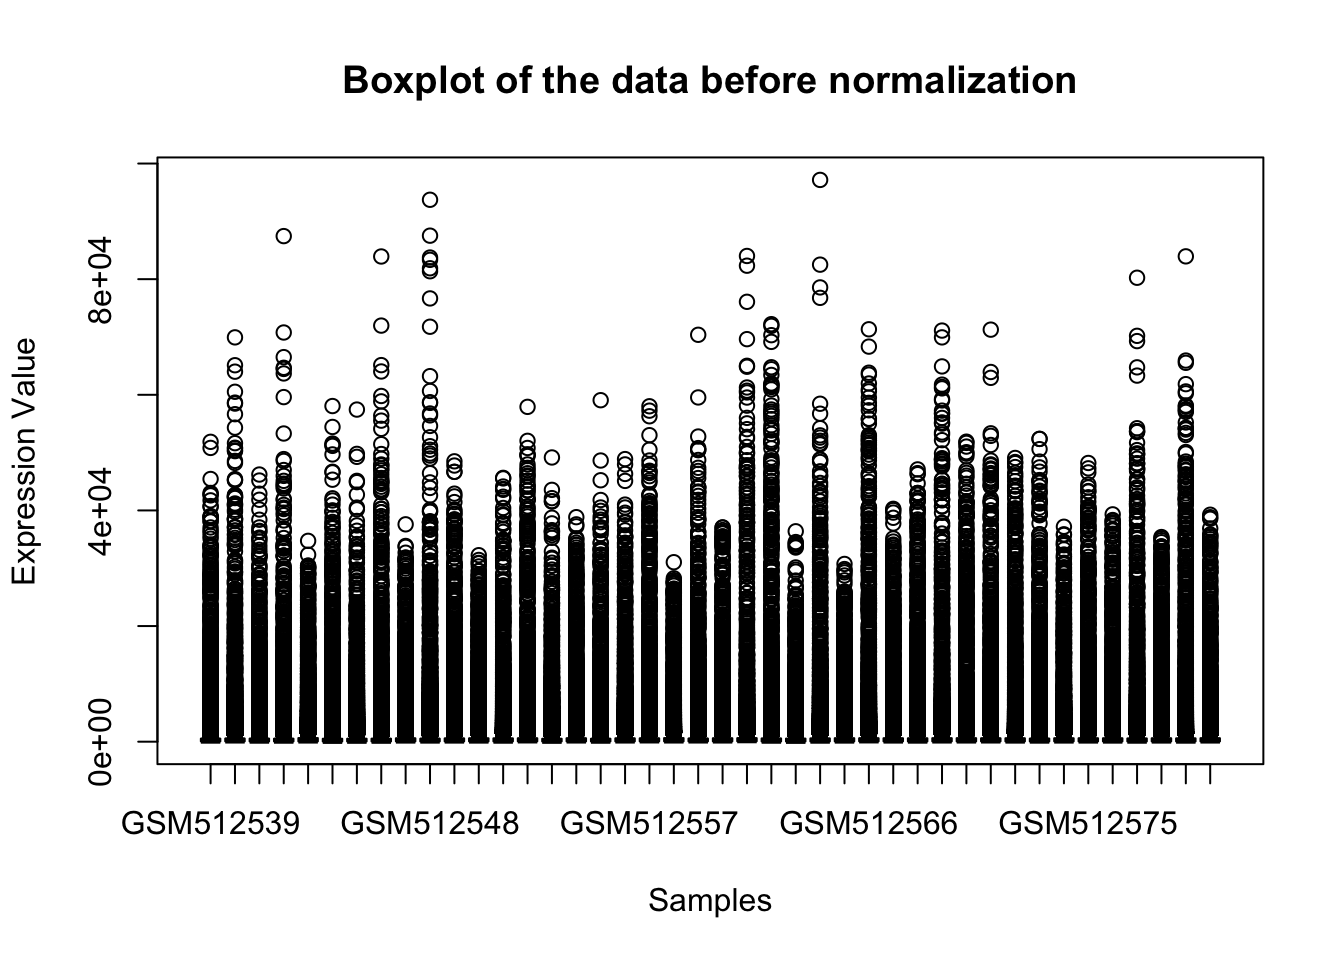
\includegraphics{NBDA_project_files/figure-latex/boxplot original data-1.pdf}

The boxplot shows that scaling is necessary. So, in this case, I try to
apply a log transformation to the data.

\begin{Shaded}
\begin{Highlighting}[]
\NormalTok{ex2}\OtherTok{\textless{}{-}}\FunctionTok{log}\NormalTok{(ex)}
\NormalTok{ex2 }\OtherTok{\textless{}{-}} \FunctionTok{na.omit}\NormalTok{(}\FunctionTok{as.matrix}\NormalTok{(ex2))}
\CommentTok{\#dim(ex2) \# 22283    42 same as before}
\FunctionTok{boxplot}\NormalTok{(ex2, }\AttributeTok{main =} \StringTok{\textquotesingle{}Boxplot of the data after applying a logarithmic transformation\textquotesingle{}}\NormalTok{,}
        \AttributeTok{xlab =} \StringTok{"Samples"}\NormalTok{,}
        \AttributeTok{ylab =} \StringTok{"Expression Value"}
\NormalTok{        )}
\end{Highlighting}
\end{Shaded}

\begin{figure}
\centering
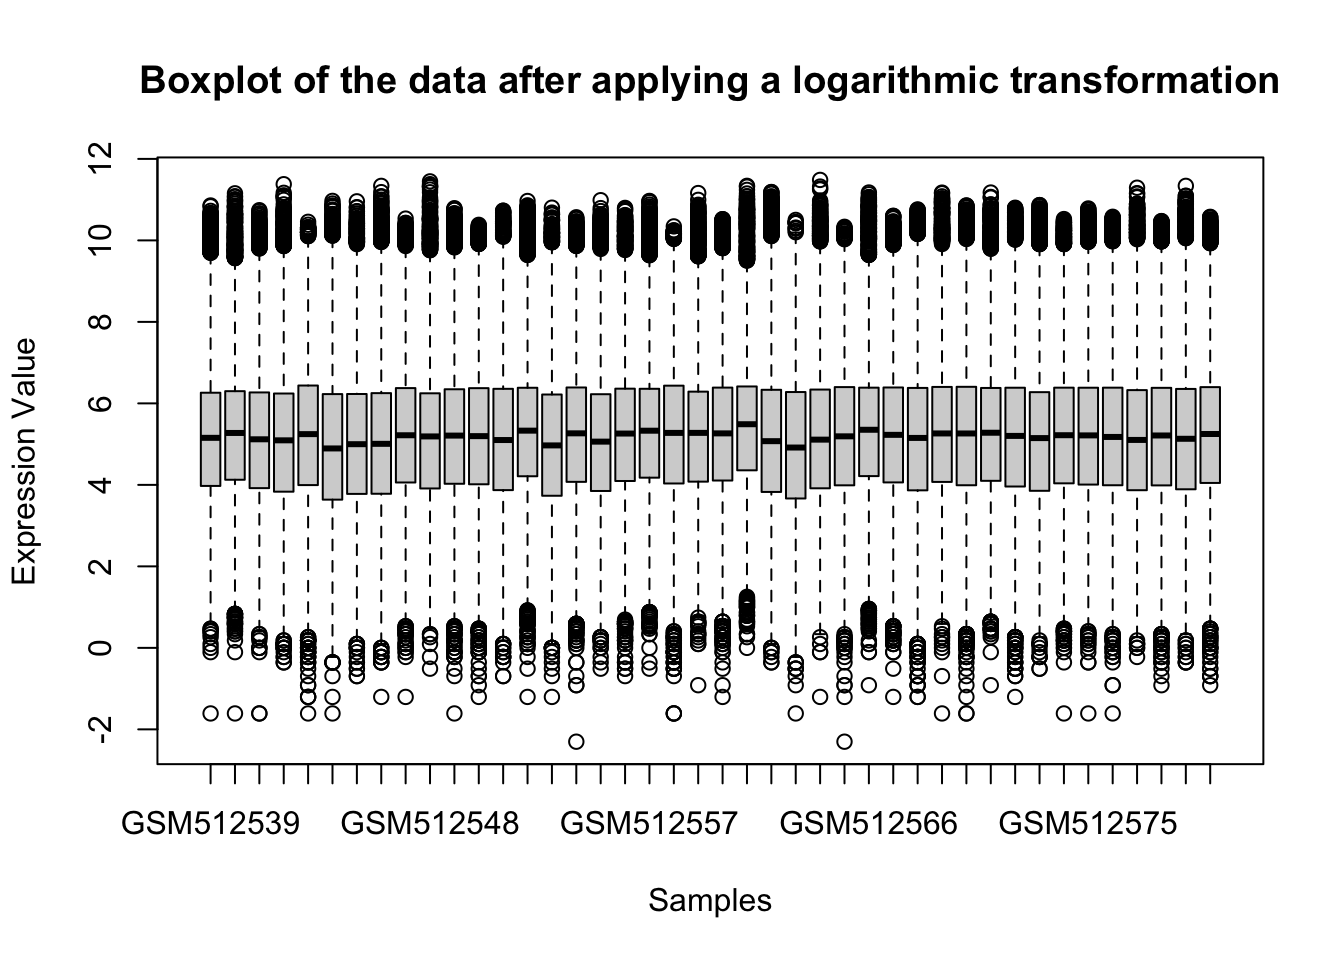
\includegraphics{NBDA_project_files/figure-latex/boxplot log transformation-1.pdf}
\caption{Boxplot of the data after applying a logarithmic
transformation}
\end{figure}

From the boxplot after the log transformation, I can see that there is
some variation in the median of the samples. So, I try to apply a median
normalization to the data after the log transformation.

\begin{Shaded}
\begin{Highlighting}[]
\CommentTok{\# MEDIAN NORMALIZATION}
\NormalTok{channel.medians}\OtherTok{=}\FunctionTok{apply}\NormalTok{(}\FunctionTok{log}\NormalTok{(ex),}\DecValTok{2}\NormalTok{,median)}
\NormalTok{normalized.log.ex}\OtherTok{=}\FunctionTok{sweep}\NormalTok{(}\FunctionTok{log}\NormalTok{(ex),}\DecValTok{2}\NormalTok{,channel.medians,}\StringTok{"{-}"}\NormalTok{)}

\CommentTok{\# boxplot post median normalization on ex}
\FunctionTok{boxplot}\NormalTok{(normalized.log.ex, }
        \AttributeTok{main =} \StringTok{\textquotesingle{}Boxplot of the data after median normalization\textquotesingle{}}\NormalTok{,}
        \AttributeTok{xlab =} \StringTok{"Samples"}\NormalTok{,}
        \AttributeTok{ylab =} \StringTok{"Expression Value"}\NormalTok{)}
\end{Highlighting}
\end{Shaded}

\begin{figure}
\centering
\includegraphics{NBDA_project_files/figure-latex/median normalization and boxplot-1.pdf}
\caption{Boxplot of the data after median normalization}
\end{figure}

\subsection{PCA}\label{pca}

PCA is a dimensionality reduction technique that allows to condense
thousands of dimensions into just two or three. For the dataset's
samples, the PCA scores display the coordinates in relation to these
additional dimensions.

\begin{Shaded}
\begin{Highlighting}[]
\NormalTok{pca }\OtherTok{\textless{}{-}} \FunctionTok{prcomp}\NormalTok{(}\FunctionTok{t}\NormalTok{(normalized.log.ex))}

\FunctionTok{summary}\NormalTok{(pca)}
\end{Highlighting}
\end{Shaded}

\begin{verbatim}
## Importance of components:
##                            PC1      PC2      PC3      PC4      PC5      PC6      PC7      PC8      PC9     PC10
## Standard deviation     38.8020 23.47065 20.63892 19.54327 18.43330 15.97431 15.54787 15.25339 14.95988 13.82648
## Proportion of Variance  0.1791  0.06552  0.05067  0.04543  0.04042  0.03035  0.02875  0.02767  0.02662  0.02274
## Cumulative Proportion   0.1791  0.24461  0.29527  0.34070  0.38112  0.41147  0.44023  0.46790  0.49452  0.51726
##                            PC11     PC12     PC13     PC14     PC15     PC16     PC17     PC18     PC19     PC20
## Standard deviation     13.67761 13.63388 13.39954 13.05683 12.96288 12.78929 12.64910 12.48152 12.32645 12.13869
## Proportion of Variance  0.02225  0.02211  0.02136  0.02028  0.01999  0.01946  0.01903  0.01853  0.01807  0.01753
## Cumulative Proportion   0.53951  0.56162  0.58298  0.60326  0.62324  0.64270  0.66173  0.68026  0.69833  0.71586
##                            PC21     PC22     PC23     PC24     PC25     PC26     PC27     PC28     PC29     PC30
## Standard deviation     12.04722 11.97088 11.90374 11.69483 11.60734 11.57222 11.46507 11.15870 11.04915 10.99769
## Proportion of Variance  0.01726  0.01705  0.01685  0.01627  0.01603  0.01593  0.01564  0.01481  0.01452  0.01439
## Cumulative Proportion   0.73312  0.75017  0.76702  0.78329  0.79932  0.81525  0.83088  0.84569  0.86021  0.87460
##                            PC31     PC32     PC33     PC34   PC35    PC36    PC37    PC38   PC39    PC40    PC41
## Standard deviation     10.68517 10.45191 10.25430 10.13818 9.9583 9.68456 9.50070 9.42259 9.3053 9.17335 8.95347
## Proportion of Variance  0.01358  0.01299  0.01251  0.01223 0.0118 0.01116 0.01074 0.01056 0.0103 0.01001 0.00954
## Cumulative Proportion   0.88818  0.90117  0.91368  0.92591 0.9377 0.94886 0.95960 0.97016 0.9805 0.99046 1.00000
##                             PC42
## Standard deviation     6.784e-14
## Proportion of Variance 0.000e+00
## Cumulative Proportion  1.000e+00
\end{verbatim}

\begin{Shaded}
\begin{Highlighting}[]
\FunctionTok{screeplot}\NormalTok{(pca)}
\end{Highlighting}
\end{Shaded}

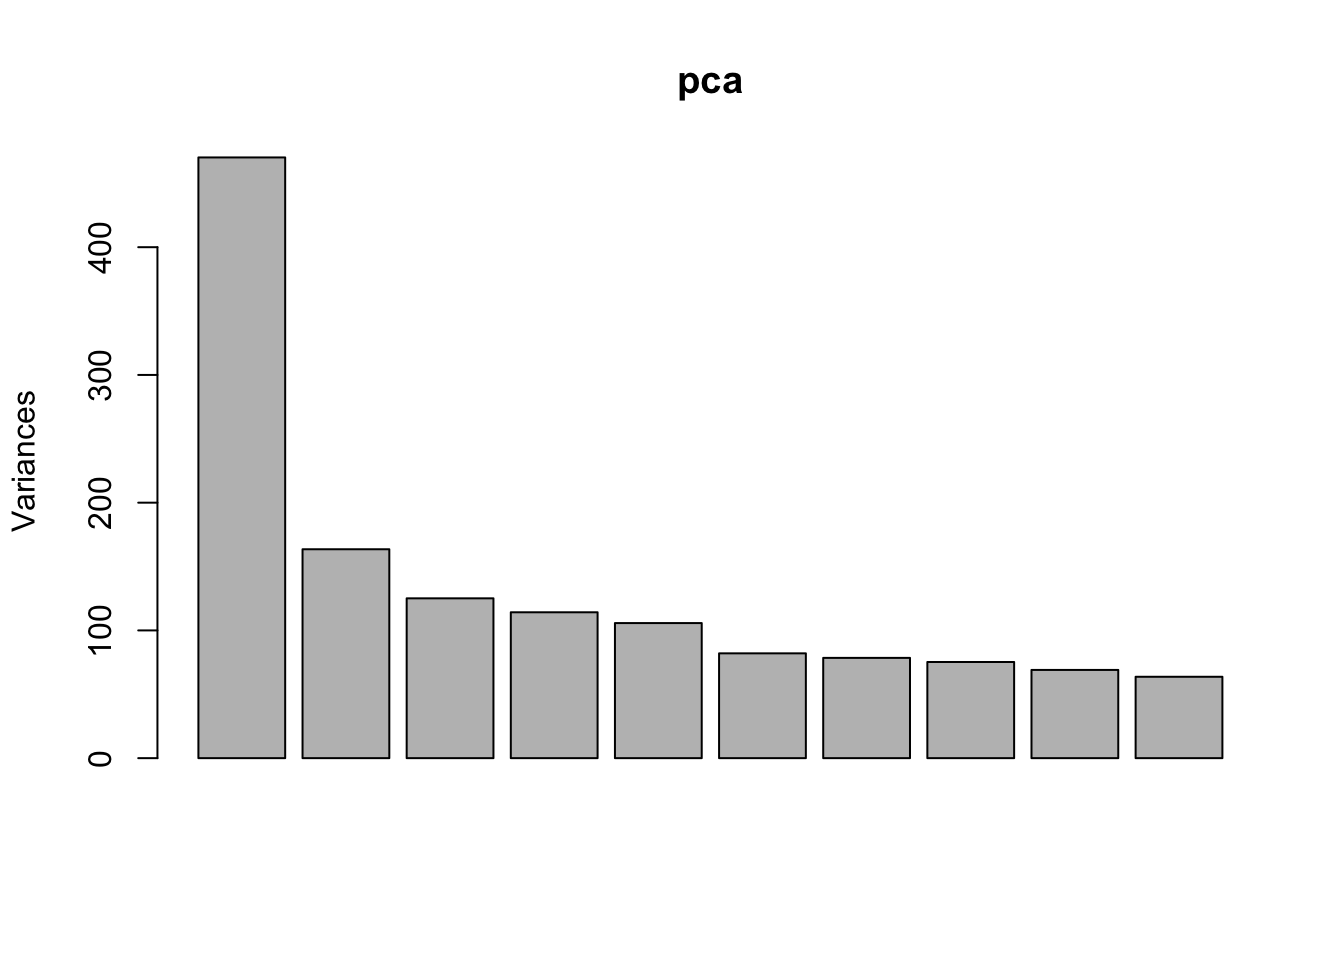
\includegraphics{NBDA_project_files/figure-latex/pca-1.pdf}

To get the summary of the PCA and the plot showing the variance
explained by the first 10 components, it is possible to use the
functions commented in the chunks above.

However, using \texttt{ggplot2} and \texttt{factoextra} packages is
possible to get a more concise and informative plot reporting the same
information.

\begin{Shaded}
\begin{Highlighting}[]
\NormalTok{pcaVar }\OtherTok{\textless{}{-}} \FunctionTok{get\_eig}\NormalTok{(pca)}
\NormalTok{pcaVar }\OtherTok{\textless{}{-}}\NormalTok{ pcaVar}\SpecialCharTok{$}\NormalTok{variance.percent[}\DecValTok{1}\SpecialCharTok{:}\DecValTok{10}\NormalTok{]}
\NormalTok{screeDf }\OtherTok{\textless{}{-}} \FunctionTok{data.frame}\NormalTok{(}\StringTok{"Dimensions"} \OtherTok{=} \FunctionTok{as.factor}\NormalTok{(}\FunctionTok{seq}\NormalTok{(}\DecValTok{1}\NormalTok{,}\DecValTok{10}\NormalTok{)),}
                      \StringTok{"Percentages"} \OtherTok{=}\NormalTok{ pcaVar,}
                      \StringTok{"Labels"} \OtherTok{=} \FunctionTok{paste}\NormalTok{(}\FunctionTok{round}\NormalTok{(pcaVar, }\DecValTok{2}\NormalTok{), }\StringTok{"\%"}\NormalTok{))}

\NormalTok{p }\OtherTok{\textless{}{-}} \FunctionTok{ggplot}\NormalTok{(}\AttributeTok{data =}\NormalTok{ screeDf, }\FunctionTok{aes}\NormalTok{(}\AttributeTok{x=}\NormalTok{Dimensions, }\AttributeTok{y=}\NormalTok{Percentages))}\SpecialCharTok{+}
  \FunctionTok{geom\_bar}\NormalTok{(}\AttributeTok{stat =} \StringTok{"identity"}\NormalTok{, }\AttributeTok{fill =} \StringTok{"\#d1105a"}\NormalTok{)}\SpecialCharTok{+}
  \FunctionTok{geom\_text}\NormalTok{(}\FunctionTok{aes}\NormalTok{(}\AttributeTok{label=}\NormalTok{Labels), }\AttributeTok{vjust=}\SpecialCharTok{{-}}\FloatTok{0.5}\NormalTok{, }\AttributeTok{color=}\StringTok{"black"}\NormalTok{, }\AttributeTok{size=}\FloatTok{3.6}\NormalTok{)}\SpecialCharTok{+}
  \FunctionTok{ggtitle}\NormalTok{(}\StringTok{"Scree Plot"}\NormalTok{)}\SpecialCharTok{+}
  \FunctionTok{ylab}\NormalTok{(}\StringTok{"Percentage of variance explained"}\NormalTok{)}\SpecialCharTok{+}
  \FunctionTok{scale\_x\_discrete}\NormalTok{(}\AttributeTok{labels =} \FunctionTok{as.factor}\NormalTok{(}\FunctionTok{seq}\NormalTok{(}\DecValTok{1}\NormalTok{,}\DecValTok{10}\NormalTok{)))}
\NormalTok{p}
\end{Highlighting}
\end{Shaded}

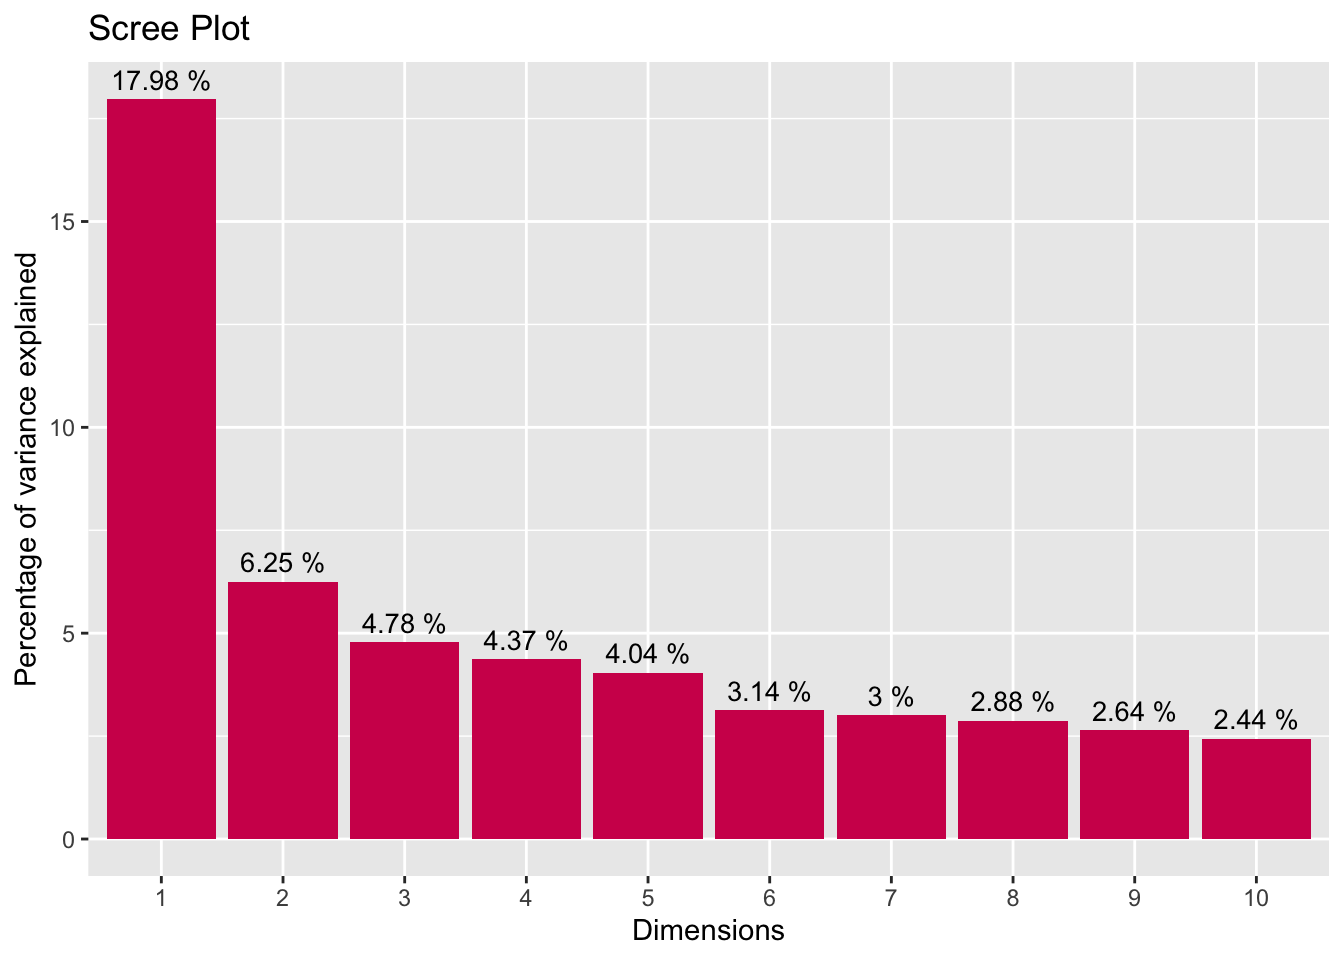
\includegraphics{NBDA_project_files/figure-latex/variance explained by pca-1.pdf}

The scree plot shows that the first dimensions on the left are the more
important because the percentage of variance explained by them is
higher. The remaining principal components account for a very small
proportion of the variability and are probably unimportant.

Let's try to plot the PCA, looking if we can see a separation between
Control and Breast Cancer groups.

\begin{Shaded}
\begin{Highlighting}[]
\CommentTok{\# draw PCA plot control VS breast cancer}
\NormalTok{group }\OtherTok{\textless{}{-}} \FunctionTok{c}\NormalTok{(}\FunctionTok{rep}\NormalTok{(}\StringTok{"cadetblue1"}\NormalTok{,}\DecValTok{18}\NormalTok{), }\FunctionTok{rep}\NormalTok{(}\StringTok{"red"}\NormalTok{,}\DecValTok{18}\NormalTok{), }\FunctionTok{rep}\NormalTok{(}\StringTok{"cadetblue1"}\NormalTok{,}\DecValTok{6}\NormalTok{) ) }
\FunctionTok{plot}\NormalTok{(pca}\SpecialCharTok{$}\NormalTok{x[,}\DecValTok{1}\NormalTok{], pca}\SpecialCharTok{$}\NormalTok{x[,}\DecValTok{2}\NormalTok{], }\AttributeTok{xlab=}\StringTok{"PCA1"}\NormalTok{, }\AttributeTok{ylab=}\StringTok{"PCA2"}\NormalTok{, }\AttributeTok{main=}\StringTok{"PCA for components 1 and 2"}\NormalTok{, }\AttributeTok{type=}\StringTok{"p"}\NormalTok{, }\AttributeTok{pch=}\DecValTok{10}\NormalTok{, }\AttributeTok{col=}\NormalTok{group)}
\FunctionTok{text}\NormalTok{(pca}\SpecialCharTok{$}\NormalTok{x[,}\DecValTok{1}\NormalTok{], pca}\SpecialCharTok{$}\NormalTok{x[,}\DecValTok{2}\NormalTok{], }\FunctionTok{rownames}\NormalTok{(pca}\SpecialCharTok{$}\NormalTok{data), }\AttributeTok{cex=}\FloatTok{0.75}\NormalTok{)}
\FunctionTok{legend}\NormalTok{(}\StringTok{"topleft"}\NormalTok{, }\AttributeTok{col=}\FunctionTok{c}\NormalTok{(}\StringTok{"cadetblue1"}\NormalTok{,}\StringTok{"red"}\NormalTok{), }\AttributeTok{legend =} \FunctionTok{c}\NormalTok{(}\StringTok{"Control"}\NormalTok{, }\StringTok{"Breast Cancer"}\NormalTok{),}
    \AttributeTok{pch =} \DecValTok{20}\NormalTok{, }\AttributeTok{bty=}\StringTok{\textquotesingle{}n\textquotesingle{}}\NormalTok{, }\AttributeTok{cex=}\NormalTok{.}\DecValTok{55}\NormalTok{)}
\end{Highlighting}
\end{Shaded}

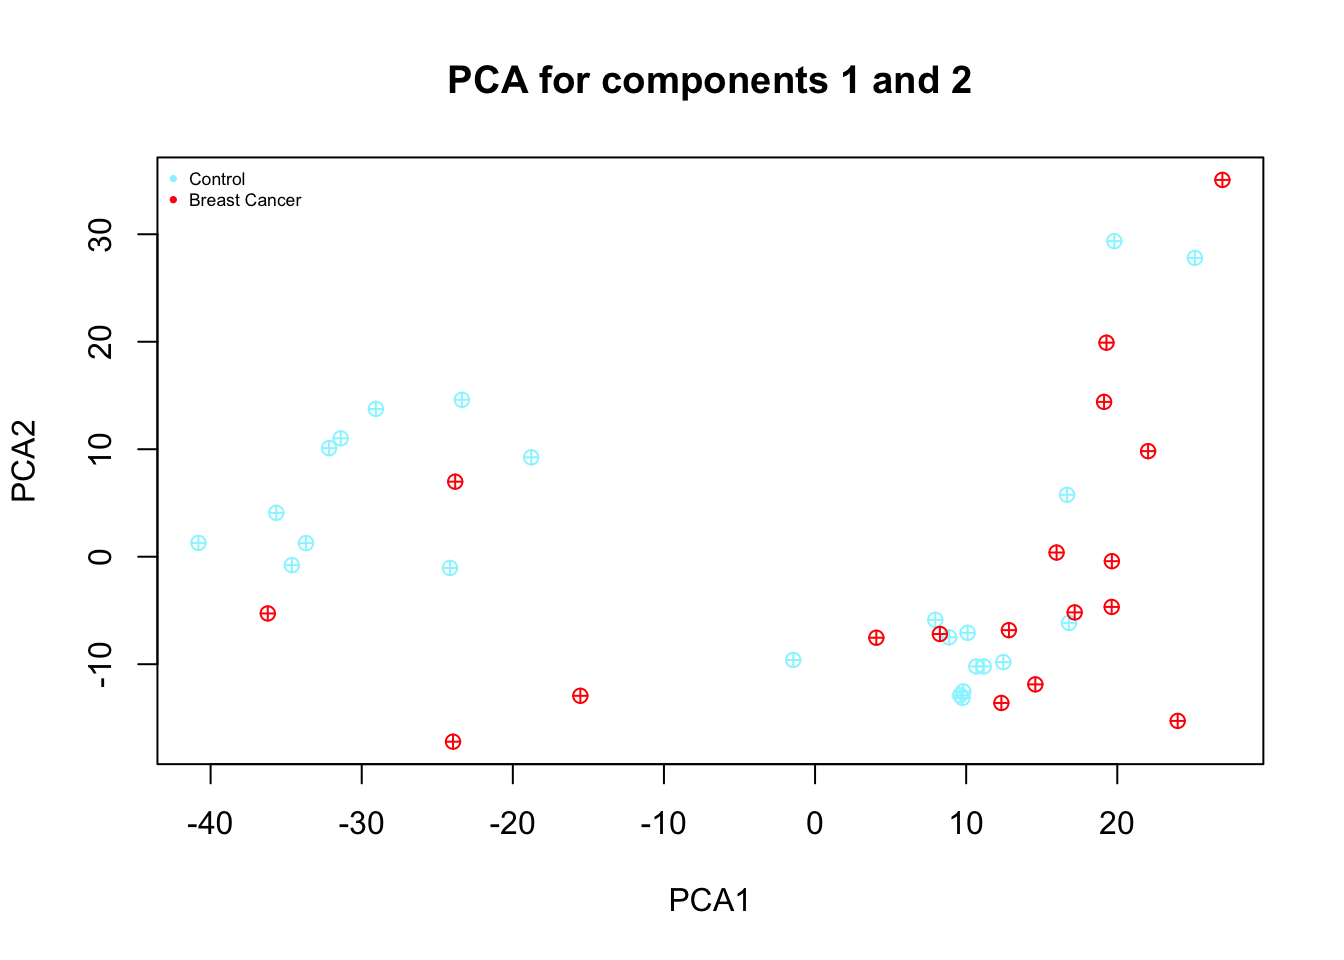
\includegraphics{NBDA_project_files/figure-latex/PCA for components 1 and 2 control VS Breast cancer without labels-1.pdf}

Let's try to add the control subtypes. The vector group used in the PCA
plot is based on the data. The samples corresponding to the colors are
the following:

\begin{itemize}
\item
  \textbf{Light blue}: reduction mammoplasty (RM) breast epithelium
  samples
\item
  \textbf{Red}: histologically normal (HN) epithelial samples from
  breast cancer patient
\item
  \textbf{Purple}: histologically normal breast epithelium (NlEpi) from
  prophylactic mastectomy patient samples
\end{itemize}

\begin{Shaded}
\begin{Highlighting}[]
\CommentTok{\# draw PCA plot}
\NormalTok{group }\OtherTok{\textless{}{-}} \FunctionTok{c}\NormalTok{(}\FunctionTok{rep}\NormalTok{(}\StringTok{"cadetblue1"}\NormalTok{,}\DecValTok{18}\NormalTok{), }\FunctionTok{rep}\NormalTok{(}\StringTok{"red"}\NormalTok{,}\DecValTok{18}\NormalTok{), }\FunctionTok{rep}\NormalTok{(}\StringTok{"purple"}\NormalTok{,}\DecValTok{6}\NormalTok{) ) }\CommentTok{\# vector of colors based on the order of my data}
\FunctionTok{plot}\NormalTok{(pca}\SpecialCharTok{$}\NormalTok{x[,}\DecValTok{1}\NormalTok{], pca}\SpecialCharTok{$}\NormalTok{x[,}\DecValTok{2}\NormalTok{], }\AttributeTok{xlab=}\StringTok{"PCA1"}\NormalTok{, }\AttributeTok{ylab=}\StringTok{"PCA2"}\NormalTok{, }\AttributeTok{main=}\StringTok{"PCA for components 1 and 2"}\NormalTok{, }\AttributeTok{type=}\StringTok{"p"}\NormalTok{, }\AttributeTok{pch=}\DecValTok{10}\NormalTok{, }\AttributeTok{col=}\NormalTok{group)}
\FunctionTok{text}\NormalTok{(pca}\SpecialCharTok{$}\NormalTok{x[,}\DecValTok{1}\NormalTok{], pca}\SpecialCharTok{$}\NormalTok{x[,}\DecValTok{2}\NormalTok{], }\FunctionTok{rownames}\NormalTok{(pca}\SpecialCharTok{$}\NormalTok{data), }\AttributeTok{cex=}\FloatTok{0.75}\NormalTok{)}
\FunctionTok{legend}\NormalTok{(}\StringTok{"topleft"}\NormalTok{, }\AttributeTok{col=}\FunctionTok{c}\NormalTok{(}\StringTok{"cadetblue1"}\NormalTok{,}\StringTok{"red"}\NormalTok{,}\StringTok{"purple"}\NormalTok{), }\AttributeTok{legend =} \FunctionTok{c}\NormalTok{(}\StringTok{"Reduction Mammoplasty"}\NormalTok{, }\StringTok{"Breast Cancer"}\NormalTok{, }\StringTok{"Prophylactic Mastectomy"}\NormalTok{),}
    \AttributeTok{pch =} \DecValTok{20}\NormalTok{, }\AttributeTok{bty=}\StringTok{\textquotesingle{}n\textquotesingle{}}\NormalTok{, }\AttributeTok{cex=}\NormalTok{.}\DecValTok{55}\NormalTok{)}
\end{Highlighting}
\end{Shaded}

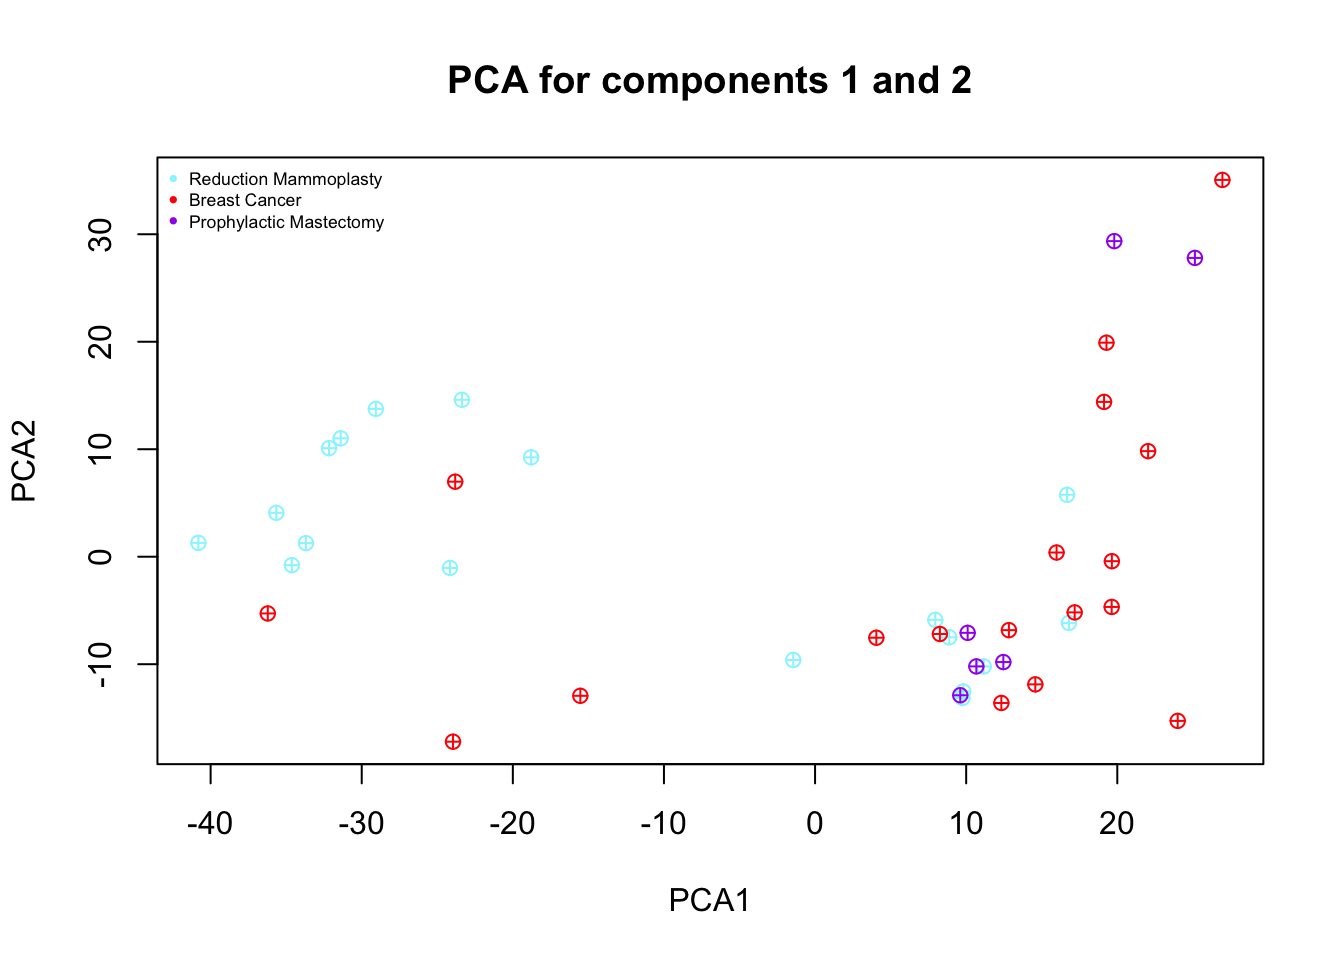
\includegraphics{NBDA_project_files/figure-latex/PCA for components 1 and 2 control subtypes without labels-1.pdf}

Then, I try to see if there is a separation also inside different types
of Breast Cancer.

\begin{Shaded}
\begin{Highlighting}[]
\CommentTok{\# draw PCA plot with all subtypes}
\NormalTok{group }\OtherTok{\textless{}{-}} \FunctionTok{c}\NormalTok{(}\FunctionTok{rep}\NormalTok{(my\_colors[}\DecValTok{7}\NormalTok{],}\DecValTok{18}\NormalTok{), }\FunctionTok{rep}\NormalTok{(my\_colors[}\DecValTok{4}\NormalTok{],}\DecValTok{9}\NormalTok{), }\FunctionTok{rep}\NormalTok{(my\_colors[}\DecValTok{1}\NormalTok{],}\DecValTok{9}\NormalTok{), }\FunctionTok{rep}\NormalTok{(my\_colors[}\DecValTok{6}\NormalTok{],}\DecValTok{6}\NormalTok{) ) }\CommentTok{\# vector of colors based on the order of my data}
\FunctionTok{plot}\NormalTok{(pca}\SpecialCharTok{$}\NormalTok{x[,}\DecValTok{1}\NormalTok{], pca}\SpecialCharTok{$}\NormalTok{x[,}\DecValTok{2}\NormalTok{], }\AttributeTok{xlab=}\StringTok{"PCA1"}\NormalTok{, }\AttributeTok{ylab=}\StringTok{"PCA2"}\NormalTok{, }\AttributeTok{main=}\StringTok{"PCA for components 1 and 2"}\NormalTok{, }\AttributeTok{type=}\StringTok{"p"}\NormalTok{, }\AttributeTok{pch=}\DecValTok{10}\NormalTok{, }\AttributeTok{col=}\NormalTok{group)}
\FunctionTok{text}\NormalTok{(pca}\SpecialCharTok{$}\NormalTok{x[,}\DecValTok{1}\NormalTok{], pca}\SpecialCharTok{$}\NormalTok{x[,}\DecValTok{2}\NormalTok{], }\FunctionTok{rownames}\NormalTok{(pca}\SpecialCharTok{$}\NormalTok{data), }\AttributeTok{cex=}\FloatTok{0.75}\NormalTok{)}
\FunctionTok{legend}\NormalTok{(}\StringTok{"topleft"}\NormalTok{, }\AttributeTok{col=}\FunctionTok{c}\NormalTok{(my\_colors[}\DecValTok{7}\NormalTok{],my\_colors[}\DecValTok{4}\NormalTok{],my\_colors[}\DecValTok{1}\NormalTok{],my\_colors[}\DecValTok{6}\NormalTok{]), }\AttributeTok{legend =} \FunctionTok{c}\NormalTok{(}\StringTok{"Reduction Mammoplasty"}\NormalTok{, }\StringTok{"ER+ Breast Cancer"}\NormalTok{, }\StringTok{"ER{-} Breast Cancer"}\NormalTok{, }\StringTok{"Prophylactic Mastectomy"}\NormalTok{),}
    \AttributeTok{pch =} \DecValTok{20}\NormalTok{, }\AttributeTok{bty=}\StringTok{\textquotesingle{}n\textquotesingle{}}\NormalTok{, }\AttributeTok{cex=}\NormalTok{.}\DecValTok{55}\NormalTok{)}
\end{Highlighting}
\end{Shaded}

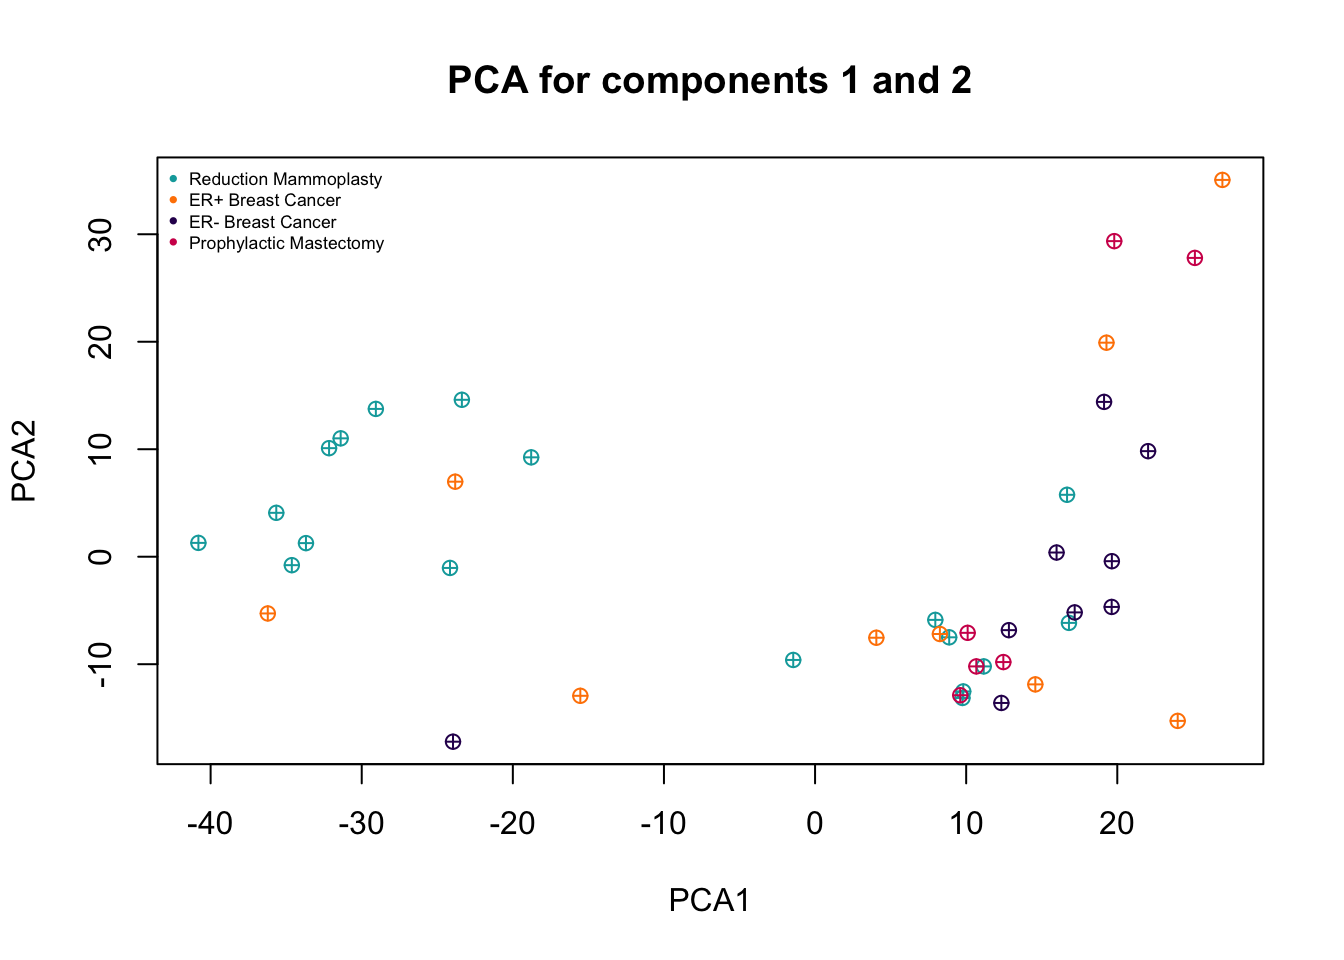
\includegraphics{NBDA_project_files/figure-latex/pca with all subtypes without labels-1.pdf}

\subsubsection{Interactive PCA plot}\label{interactive-pca-plot}

Let's try to explore an interactive PCA plot.

\begin{Shaded}
\begin{Highlighting}[]
\NormalTok{components}\OtherTok{\textless{}{-}}\NormalTok{pca[[}\StringTok{"x"}\NormalTok{]]}
\NormalTok{components}\OtherTok{\textless{}{-}}\FunctionTok{data.frame}\NormalTok{(components)}
\NormalTok{type}\OtherTok{\textless{}{-}}\FunctionTok{c}\NormalTok{(}\FunctionTok{rep}\NormalTok{(}\StringTok{"RM"}\NormalTok{, }\DecValTok{18}\NormalTok{), }\FunctionTok{rep}\NormalTok{(}\StringTok{"HN"}\NormalTok{,}\DecValTok{18}\NormalTok{), }\FunctionTok{rep}\NormalTok{(}\StringTok{"NlEpi"}\NormalTok{,}\DecValTok{6}\NormalTok{))}
\NormalTok{components}\OtherTok{\textless{}{-}}\FunctionTok{cbind}\NormalTok{(components, type )}

\NormalTok{fig }\OtherTok{\textless{}{-}} \FunctionTok{plot\_ly}\NormalTok{(components, }\AttributeTok{x=}\SpecialCharTok{\textasciitilde{}}\NormalTok{PC1, }\AttributeTok{y=}\SpecialCharTok{\textasciitilde{}}\NormalTok{PC2, }
               \AttributeTok{color=}\NormalTok{type,}\AttributeTok{colors=}\FunctionTok{c}\NormalTok{(}\StringTok{\textquotesingle{}cadetblue1\textquotesingle{}}\NormalTok{, }\StringTok{\textquotesingle{}red\textquotesingle{}}\NormalTok{,}\StringTok{\textquotesingle{}purple\textquotesingle{}}\NormalTok{), }
               \AttributeTok{type=}\StringTok{\textquotesingle{}scatter\textquotesingle{}}\NormalTok{,}\AttributeTok{mode=}\StringTok{\textquotesingle{}markers\textquotesingle{}}\NormalTok{)}
\NormalTok{fig}
\end{Highlighting}
\end{Shaded}

\begin{Shaded}
\begin{Highlighting}[]
\NormalTok{fig2 }\OtherTok{\textless{}{-}} \FunctionTok{plot\_ly}\NormalTok{(components, }\AttributeTok{x=}\SpecialCharTok{\textasciitilde{}}\NormalTok{PC1, }\AttributeTok{y=}\SpecialCharTok{\textasciitilde{}}\NormalTok{PC2, }\AttributeTok{z=}\SpecialCharTok{\textasciitilde{}}\NormalTok{PC3, }
                \AttributeTok{color=}\NormalTok{type, }\AttributeTok{colors=}\FunctionTok{c}\NormalTok{(}\StringTok{\textquotesingle{}cadetblue1\textquotesingle{}}\NormalTok{, }\StringTok{\textquotesingle{}red\textquotesingle{}}\NormalTok{,}\StringTok{\textquotesingle{}purple\textquotesingle{}}\NormalTok{),}
                \AttributeTok{mode=}\StringTok{\textquotesingle{}markers\textquotesingle{}}\NormalTok{, }\AttributeTok{marker =} \FunctionTok{list}\NormalTok{(}\AttributeTok{size =} \DecValTok{4}\NormalTok{))}
\NormalTok{fig2}
\end{Highlighting}
\end{Shaded}

\begin{Shaded}
\begin{Highlighting}[]
\NormalTok{fig3 }\OtherTok{\textless{}{-}} \FunctionTok{plot\_ly}\NormalTok{(components, }\AttributeTok{x=}\SpecialCharTok{\textasciitilde{}}\NormalTok{PC1, }\AttributeTok{y=}\SpecialCharTok{\textasciitilde{}}\NormalTok{PC3, }
                \AttributeTok{color=}\NormalTok{type, }\AttributeTok{colors=}\FunctionTok{c}\NormalTok{(}\StringTok{\textquotesingle{}cadetblue1\textquotesingle{}}\NormalTok{, }\StringTok{\textquotesingle{}red\textquotesingle{}}\NormalTok{,}\StringTok{\textquotesingle{}purple\textquotesingle{}}\NormalTok{),}
                \AttributeTok{type=}\StringTok{\textquotesingle{}scatter\textquotesingle{}}\NormalTok{,}\AttributeTok{mode=}\StringTok{\textquotesingle{}markers\textquotesingle{}}\NormalTok{)}
\NormalTok{fig3}
\end{Highlighting}
\end{Shaded}

\subsection{UMAP}\label{umap}

\begin{Shaded}
\begin{Highlighting}[]
\NormalTok{umap\_data }\OtherTok{\textless{}{-}}\NormalTok{ umap}\SpecialCharTok{::}\FunctionTok{umap}\NormalTok{(}\FunctionTok{t}\NormalTok{(normalized.log.ex), }
                        \AttributeTok{n\_neighbors =} \FunctionTok{sqrt}\NormalTok{(}\FunctionTok{dim}\NormalTok{(}\FunctionTok{t}\NormalTok{(normalized.log.ex))[}\DecValTok{1}\NormalTok{]),}\CommentTok{\#or the square root of the rows }
                        \AttributeTok{min\_dist =} \FloatTok{0.1}\NormalTok{,         }
                        \AttributeTok{metric =} \StringTok{"euclidean"}\NormalTok{,    }\CommentTok{\#you can change it}
                        \AttributeTok{n\_components =} \DecValTok{2}\NormalTok{) }\CommentTok{\#used the default ones! }

\NormalTok{umap\_df }\OtherTok{\textless{}{-}} \FunctionTok{data.frame}\NormalTok{(umap\_data}\SpecialCharTok{$}\NormalTok{layout)}
\NormalTok{group\_data }\OtherTok{\textless{}{-}} \FunctionTok{data.frame}\NormalTok{(metadata}\SpecialCharTok{$}\NormalTok{specimen.ch1)}
\NormalTok{umap\_df }\OtherTok{\textless{}{-}} \FunctionTok{cbind}\NormalTok{(umap\_df,group\_data)}
\FunctionTok{colnames}\NormalTok{(umap\_df) }\OtherTok{\textless{}{-}} \FunctionTok{c}\NormalTok{(}\StringTok{"X1"}\NormalTok{, }\StringTok{"X2"}\NormalTok{, }\StringTok{"Group"}\NormalTok{)}

\NormalTok{umap\_df}\SpecialCharTok{$}\NormalTok{Group}\OtherTok{\textless{}{-}}\FunctionTok{c}\NormalTok{(}\FunctionTok{rep}\NormalTok{(}\StringTok{"Reduction Mammoplasty"}\NormalTok{, }\DecValTok{18}\NormalTok{), }\FunctionTok{rep}\NormalTok{(}\StringTok{"ER+ Breast Cancer"}\NormalTok{,}\DecValTok{9}\NormalTok{), }\FunctionTok{rep}\NormalTok{(}\StringTok{"ER{-} Breast Cancer"}\NormalTok{, }\DecValTok{9}\NormalTok{), }\FunctionTok{rep}\NormalTok{(}\StringTok{"Prophylactic Mastectomy"}\NormalTok{,}\DecValTok{6}\NormalTok{))}

\FunctionTok{library}\NormalTok{(plotly)}

\NormalTok{figUmap }\OtherTok{\textless{}{-}} \FunctionTok{plot\_ly}\NormalTok{(umap\_df, }
                 \AttributeTok{x =} \SpecialCharTok{\textasciitilde{}}\NormalTok{X1, }\AttributeTok{y =} \SpecialCharTok{\textasciitilde{}}\NormalTok{X2, }\AttributeTok{color =}\NormalTok{ umap\_df}\SpecialCharTok{$}\NormalTok{Group,}
                 \AttributeTok{colors =} \FunctionTok{c}\NormalTok{(}\StringTok{\textquotesingle{}cadetblue1\textquotesingle{}}\NormalTok{, }\StringTok{\textquotesingle{}red\textquotesingle{}}\NormalTok{,}\StringTok{\textquotesingle{}purple\textquotesingle{}}\NormalTok{),   }
                 \AttributeTok{type =} \StringTok{\textquotesingle{}scatter\textquotesingle{}}\NormalTok{,}
                 \AttributeTok{mode =} \StringTok{\textquotesingle{}markers\textquotesingle{}}\NormalTok{,}
                 \AttributeTok{size=}\DecValTok{1}\NormalTok{)}

\CommentTok{\# Display the 2D scatter plot}
\NormalTok{figUmap}
\end{Highlighting}
\end{Shaded}

\begin{Shaded}
\begin{Highlighting}[]
\NormalTok{umap\_data\_3D }\OtherTok{\textless{}{-}}\NormalTok{ umap}\SpecialCharTok{::}\FunctionTok{umap}\NormalTok{(}\FunctionTok{t}\NormalTok{(normalized.log.ex), }
                        \AttributeTok{n\_neighbors =} \FunctionTok{sqrt}\NormalTok{(}\FunctionTok{dim}\NormalTok{(}\FunctionTok{t}\NormalTok{(normalized.log.ex))[}\DecValTok{1}\NormalTok{]),}
                      \CommentTok{\#or the square root of the rows}
                        \AttributeTok{min\_dist =} \FloatTok{0.1}\NormalTok{,         }
                        \AttributeTok{metric =} \StringTok{"euclidean"}\NormalTok{,    }\CommentTok{\#you can change it}
                        \AttributeTok{n\_components =} \DecValTok{3}\NormalTok{) }\CommentTok{\#used the default ones! }

\NormalTok{umap\_df\_3D }\OtherTok{\textless{}{-}} \FunctionTok{data.frame}\NormalTok{(umap\_data\_3D}\SpecialCharTok{$}\NormalTok{layout)}
\NormalTok{group\_data }\OtherTok{\textless{}{-}} \FunctionTok{data.frame}\NormalTok{(metadata}\SpecialCharTok{$}\NormalTok{specimen.ch1)}
\NormalTok{umap\_df\_3D }\OtherTok{\textless{}{-}} \FunctionTok{cbind}\NormalTok{(umap\_df\_3D,group\_data)}
\FunctionTok{colnames}\NormalTok{(umap\_df\_3D) }\OtherTok{\textless{}{-}} \FunctionTok{c}\NormalTok{(}\StringTok{"X1"}\NormalTok{, }\StringTok{"X2"}\NormalTok{, }\StringTok{"X3"}\NormalTok{, }\StringTok{"Group"}\NormalTok{)}

\NormalTok{umap\_df\_3D}\SpecialCharTok{$}\NormalTok{Group}\OtherTok{\textless{}{-}}\FunctionTok{c}\NormalTok{(}\FunctionTok{rep}\NormalTok{(}\StringTok{"Reduction Mammoplasty"}\NormalTok{, }\DecValTok{18}\NormalTok{), }\FunctionTok{rep}\NormalTok{(}\StringTok{"ER+ Breast Cancer"}\NormalTok{,}\DecValTok{9}\NormalTok{), }\FunctionTok{rep}\NormalTok{(}\StringTok{"ER{-} Breast Cancer"}\NormalTok{, }\DecValTok{9}\NormalTok{), }\FunctionTok{rep}\NormalTok{(}\StringTok{"Prophylactic Mastectomy"}\NormalTok{,}\DecValTok{6}\NormalTok{))}

\NormalTok{figUmap\_3D }\OtherTok{\textless{}{-}} \FunctionTok{plot\_ly}\NormalTok{(umap\_df\_3D, }
                 \AttributeTok{x =} \SpecialCharTok{\textasciitilde{}}\NormalTok{X1, }\AttributeTok{y =} \SpecialCharTok{\textasciitilde{}}\NormalTok{X2, }\AttributeTok{z=}\SpecialCharTok{\textasciitilde{}}\NormalTok{X3, }\AttributeTok{color =}\NormalTok{ umap\_df\_3D}\SpecialCharTok{$}\NormalTok{Group,}
                 \AttributeTok{colors =} \FunctionTok{c}\NormalTok{(}\StringTok{\textquotesingle{}cadetblue1\textquotesingle{}}\NormalTok{, }\StringTok{\textquotesingle{}red\textquotesingle{}}\NormalTok{,}\StringTok{\textquotesingle{}purple\textquotesingle{}}\NormalTok{),   }
                 \AttributeTok{mode =} \StringTok{\textquotesingle{}markers\textquotesingle{}}\NormalTok{,}
                 \AttributeTok{size=}\DecValTok{1}\NormalTok{) }\SpecialCharTok{\%\textgreater{}\%} \FunctionTok{layout}\NormalTok{(}\AttributeTok{title =} \StringTok{\textquotesingle{}Umap 3D\textquotesingle{}}\NormalTok{)}

\CommentTok{\# Display the 3D scatter plot}
\NormalTok{figUmap\_3D}
\end{Highlighting}
\end{Shaded}

\section{Clustering}\label{clustering}

\subsection{K-means}\label{k-means}

\begin{Shaded}
\begin{Highlighting}[]
\FunctionTok{set.seed}\NormalTok{(}\DecValTok{1}\NormalTok{)}
\NormalTok{k }\OtherTok{\textless{}{-}} \DecValTok{2} \CommentTok{\# number of clusters}

\NormalTok{kmeans\_result }\OtherTok{\textless{}{-}} \FunctionTok{kmeans}\NormalTok{(}\FunctionTok{t}\NormalTok{(normalized.log.ex),k)}
\FunctionTok{table}\NormalTok{(kmeans\_result}\SpecialCharTok{$}\NormalTok{cluster) }\CommentTok{\# tells how many samples were assigned to each cluster}
\end{Highlighting}
\end{Shaded}

\begin{verbatim}
## 
##  1  2 
## 14 28
\end{verbatim}

\begin{Shaded}
\begin{Highlighting}[]
\FunctionTok{plot}\NormalTok{(kmeans\_result, }\AttributeTok{data=}\FunctionTok{t}\NormalTok{(normalized.log.ex)) }\SpecialCharTok{+} \FunctionTok{geom\_text}\NormalTok{(}\FunctionTok{aes}\NormalTok{(}\AttributeTok{label=}\NormalTok{metadata}\SpecialCharTok{$}\NormalTok{disease.state.ch1),}\AttributeTok{hjust=}\DecValTok{0}\NormalTok{,}\AttributeTok{vjust=}\DecValTok{0}\NormalTok{)}
\end{Highlighting}
\end{Shaded}

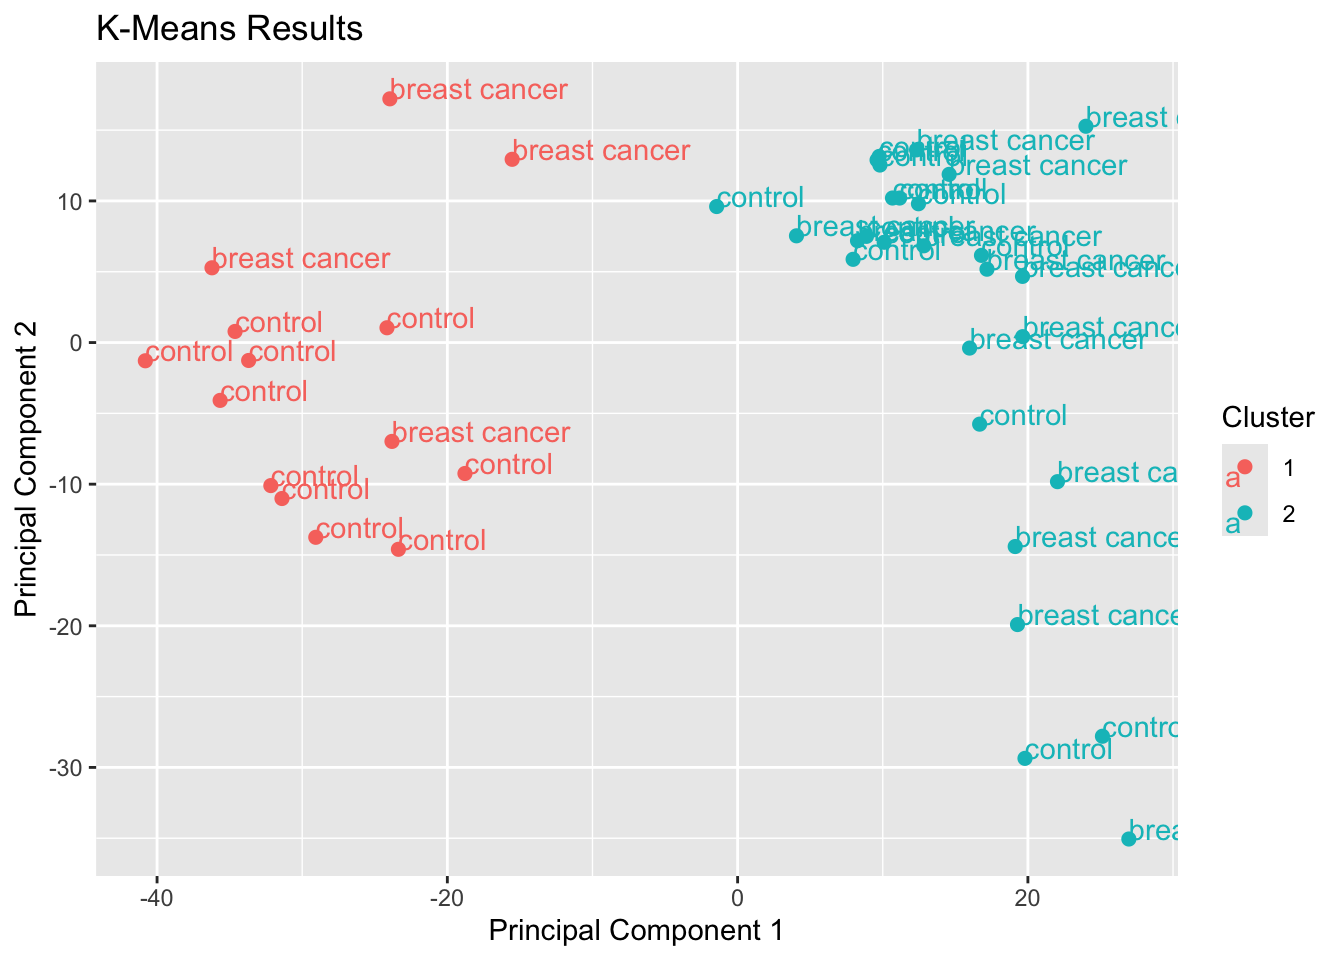
\includegraphics{NBDA_project_files/figure-latex/plot kmeans with metadata title-1.pdf}

\begin{Shaded}
\begin{Highlighting}[]
\FunctionTok{fviz\_cluster}\NormalTok{(kmeans\_result, }\AttributeTok{data =} \FunctionTok{t}\NormalTok{(normalized.log.ex),}
              \AttributeTok{palette =} \FunctionTok{c}\NormalTok{(}\StringTok{"\#FF6666"}\NormalTok{, }\StringTok{"\#33cccc"}\NormalTok{), }
             \AttributeTok{geom =} \StringTok{"point"}\NormalTok{,}
             \AttributeTok{ellipse.type =} \StringTok{"convex"}\NormalTok{, }
             \AttributeTok{ggtheme =} \FunctionTok{theme\_bw}\NormalTok{()}
\NormalTok{             )}
\end{Highlighting}
\end{Shaded}

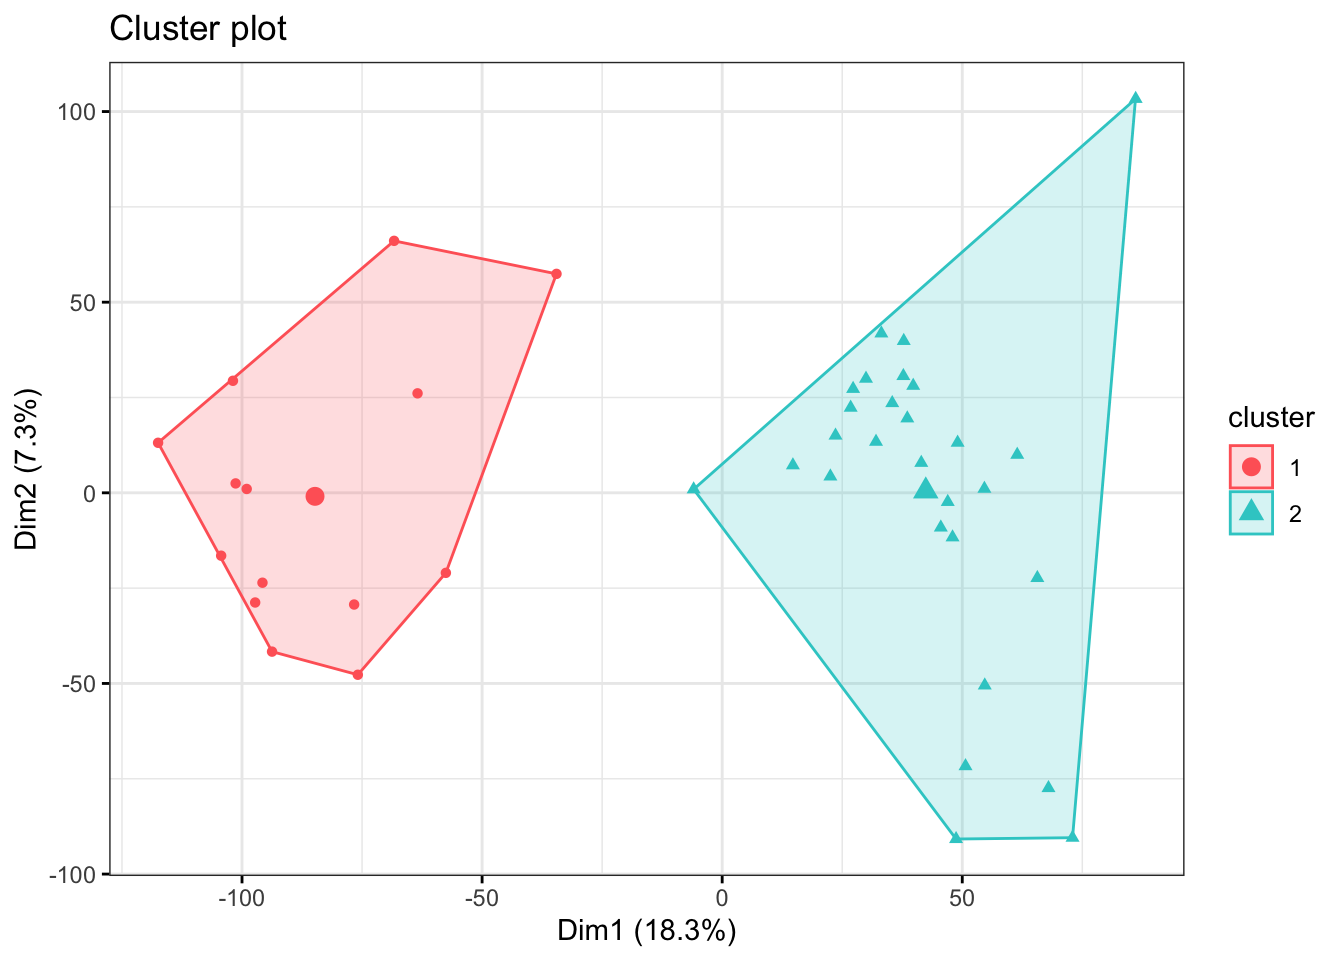
\includegraphics{NBDA_project_files/figure-latex/cluster plot kmeans 2 clusters-1.pdf}

Let's try increasing the number of clusters.

\begin{Shaded}
\begin{Highlighting}[]
\FunctionTok{set.seed}\NormalTok{(}\DecValTok{1}\NormalTok{)}
\NormalTok{k }\OtherTok{\textless{}{-}} \DecValTok{4} \CommentTok{\# number of clusters}

\NormalTok{kmeans\_result }\OtherTok{\textless{}{-}} \FunctionTok{kmeans}\NormalTok{(}\FunctionTok{t}\NormalTok{(normalized.log.ex),k)}
\FunctionTok{table}\NormalTok{(kmeans\_result}\SpecialCharTok{$}\NormalTok{cluster) }\CommentTok{\# tells how many samples were assigned to each cluster}
\end{Highlighting}
\end{Shaded}

\begin{verbatim}
## 
##  1  2  3  4 
##  8  4  6 24
\end{verbatim}

\begin{Shaded}
\begin{Highlighting}[]
\FunctionTok{plot}\NormalTok{(kmeans\_result, }\AttributeTok{data=}\FunctionTok{t}\NormalTok{(normalized.log.ex)) }\SpecialCharTok{+} \FunctionTok{geom\_text}\NormalTok{(}\FunctionTok{aes}\NormalTok{(}\AttributeTok{label=}\NormalTok{metadata}\SpecialCharTok{$}\NormalTok{specimen.ch1),}\AttributeTok{hjust=}\DecValTok{0}\NormalTok{,}\AttributeTok{vjust=}\DecValTok{0}\NormalTok{)}
\end{Highlighting}
\end{Shaded}

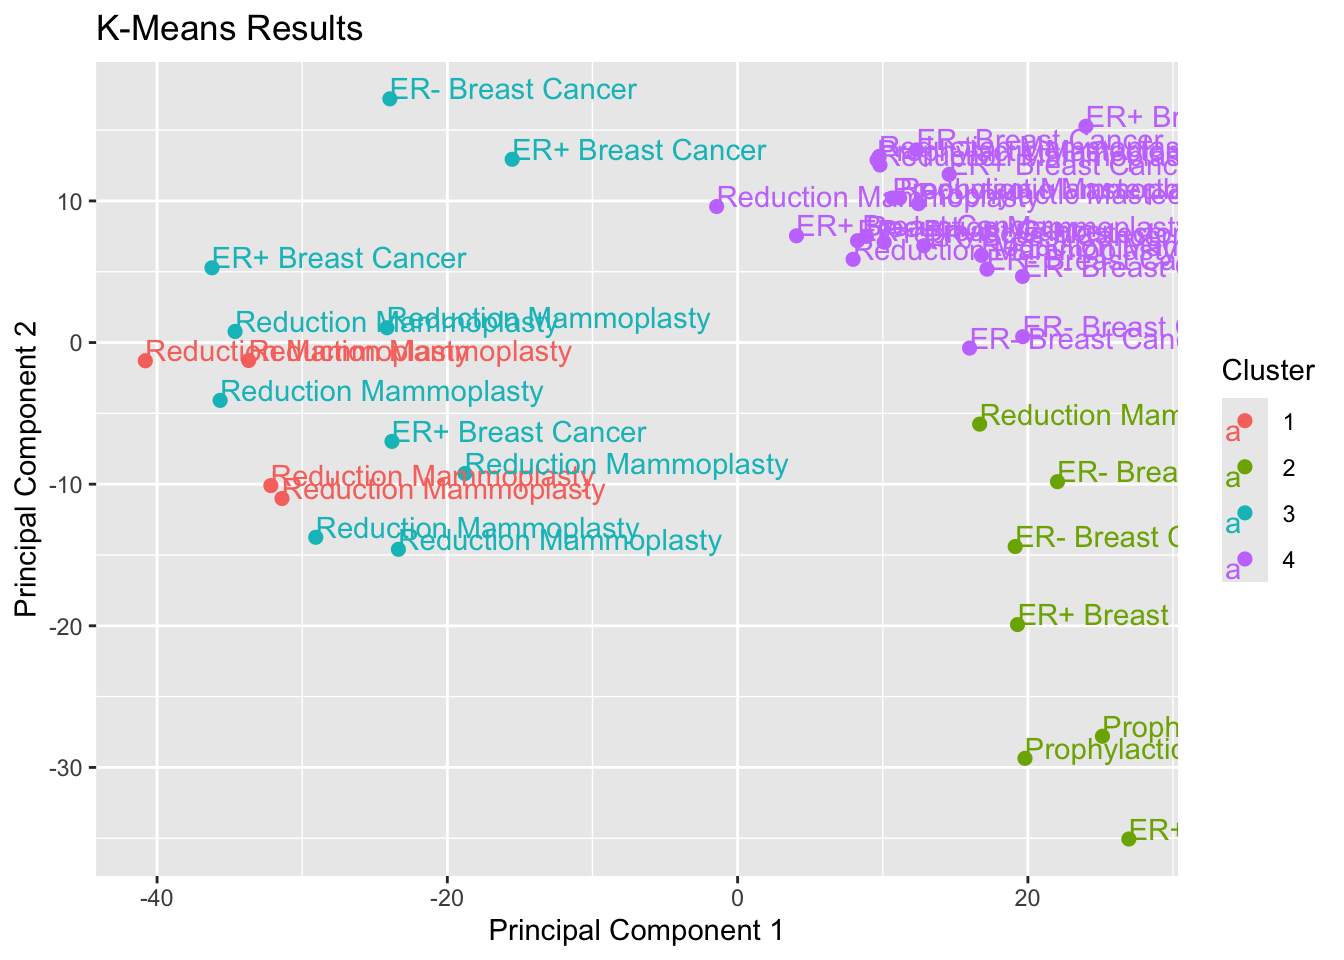
\includegraphics{NBDA_project_files/figure-latex/plot kmeans with metadata specimen-1.pdf}

\begin{Shaded}
\begin{Highlighting}[]
\FunctionTok{fviz\_cluster}\NormalTok{(kmeans\_result, }\AttributeTok{data =} \FunctionTok{t}\NormalTok{(normalized.log.ex),}
             \AttributeTok{palette =} \FunctionTok{c}\NormalTok{(}\StringTok{"\#FF6666"}\NormalTok{, }\StringTok{"\#99C666"}\NormalTok{, }\StringTok{"\#33cccc"}\NormalTok{, }\StringTok{"\#cc66ff"}\NormalTok{), }
             \AttributeTok{geom =} \StringTok{"point"}\NormalTok{,}
             \AttributeTok{ellipse.type =} \StringTok{"convex"}\NormalTok{, }
             \AttributeTok{ggtheme =} \FunctionTok{theme\_bw}\NormalTok{()}
\NormalTok{             )}
\end{Highlighting}
\end{Shaded}

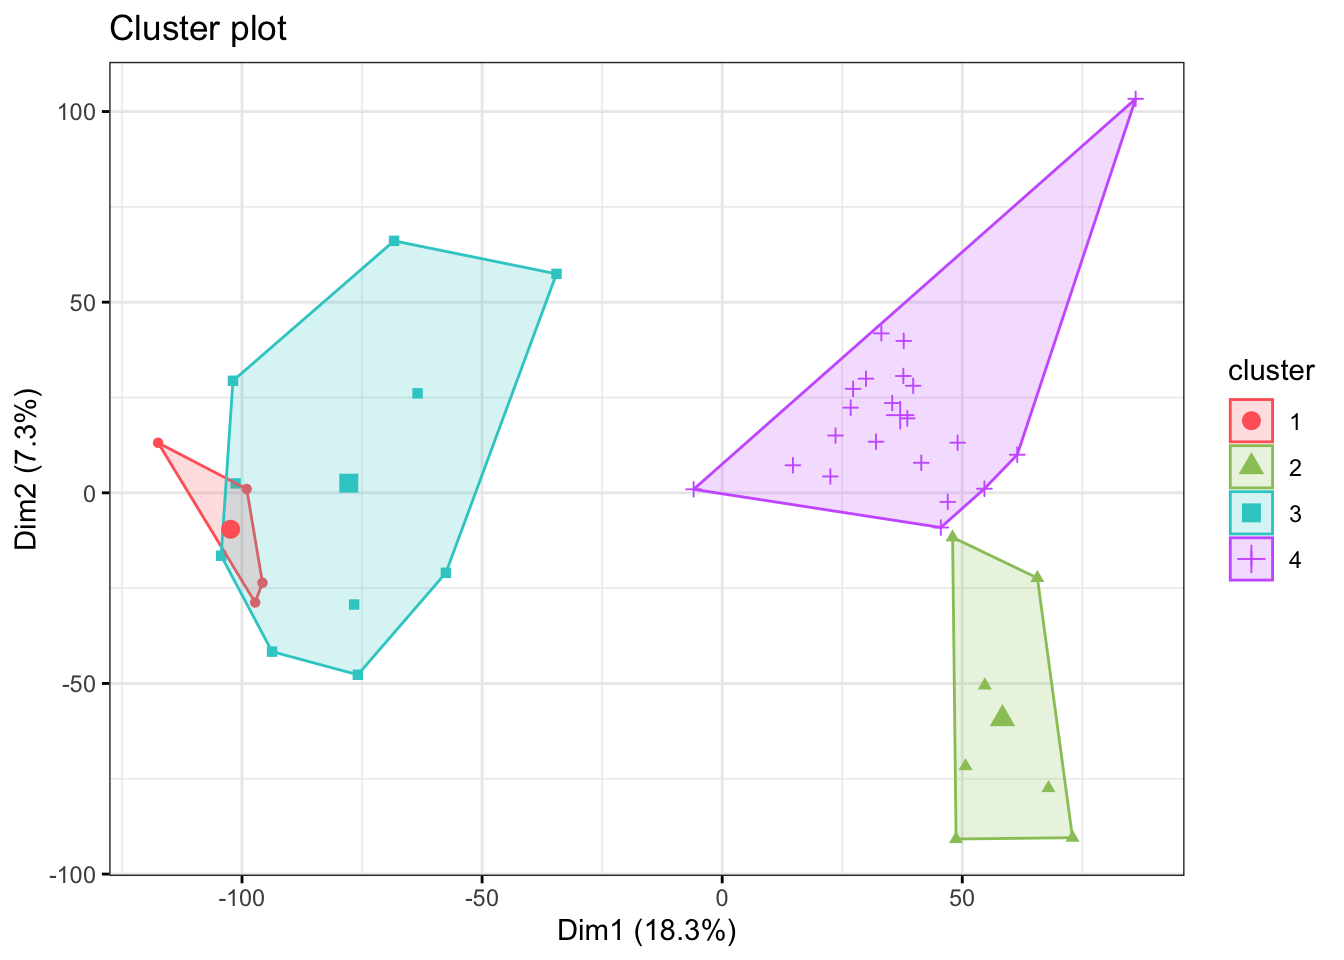
\includegraphics{NBDA_project_files/figure-latex/cluster plot kmeans 4 clusters-1.pdf}

\end{document}
